%=======================================================================
% CSE465 Final Report --- North South University
% "What an ICBHI Score Measures: A Five-Fault Evaluation Audit,
%  Corrected Baselines, and a Retracted Ceiling for Respiratory
%  Sound Classification"
%
% BUILD: pdfLaTeX on Overleaf.  Compile order: pdflatex -> bibtex -> pdflatex x2
%
% EVIDENCE RULE FOLLOWED THROUGHOUT THIS FILE
%   Every number in this document was recomputed from a committed
%   results_M*.json confusion matrix or read from a committed result file
%   in the project repository.  Nothing is transcribed from prose, and a
%   quantity that does not exist is written "not run" rather than filled
%   with a plausible value.  Source files for each table are named in the
%   table notes.
%
% FIGURES: see FIGURES_SPEC.md.  All figures referenced below exist in figures/.
%   The four data figures (inflation scatter, confusion matrix, curves, XAI
%   panels) come from the generators named in that file; the five block
%   diagrams come from `python Final_Draft/make_diagrams.py`, which reads its
%   numbers from the committed results_M*.json and never from this file.
%=======================================================================
\documentclass[journal,onecolumn]{IEEEtran}

\usepackage{graphicx}
\usepackage{amsmath}
\usepackage{amssymb}
\usepackage{booktabs}
\usepackage{multirow}
\usepackage{array}
\usepackage{url}
\usepackage[hidelinks]{hyperref}
\usepackage{algorithm}
\usepackage{algpseudocode}

\newcommand{\best}[1]{\textbf{#1}}
\newcommand{\notrun}{\textsc{not run}}

% This report carries 33 tables and 9 figures.  LaTeX holds at most 18 unprocessed
% floats at once, so the defaults below are loosened to make placement eager and
% keep the queue short.  If Overleaf ever still reports "Too many unprocessed
% floats", add \usepackage{placeins} and a \FloatBarrier at the end of the
% offending subsection -- do NOT delete a table to make it compile.
\setcounter{topnumber}{4}
\setcounter{bottomnumber}{3}
\setcounter{totalnumber}{6}
\renewcommand{\topfraction}{0.92}
\renewcommand{\bottomfraction}{0.9}
\renewcommand{\textfraction}{0.05}
\renewcommand{\floatpagefraction}{0.7}

\begin{document}

\title{What an ICBHI Score Measures: A Five-Fault Evaluation Audit,
Corrected Baselines and a Retracted Ceiling for Respiratory Sound
Classification}

\author{Asif,~Barshon~Basak,~Farhana,~and~Sami%
\thanks{The authors are with the Department of Electrical and Computer
Engineering, North South University, Dhaka, Bangladesh. Course: CSE465,
Machine Learning. Supervisor: Dr.\ Riasat Khan.}}

\maketitle

%=======================================================================
\begin{abstract}
Respiratory sound classification on the open access lung sound benchmark released
for the challenge of two thousand seventeen is a crowded field, and almost every
published system is judged by one headline score. This work asks a prior question:
how much of that score belongs to the model and how much to the way it was
measured. We audit our own pipeline of thirty nine experiments and report five
measurement faults, each recovered from a stored confusion matrix rather than
asserted, and we price each. A wrongly averaged score variant inflated twenty runs
by nine and a half points on average and twenty two at worst. A silently
substituted patient rule produced a test partition of eleven patients while
recording itself as the official one, worth nearly nine points. The published
partition assigns recordings rather than patients, so two patients appear on both
sides, although repairing that leak moves the score by four tenths of a point. The
same file names a recording whose device suffix does not match the released audio,
so a naive join discards it silently. Selecting the saved model on training loss
rather than the challenge score costs seven to ten points across three seeds.
Under the corrected protocol we segment every breathing cycle, convert it to a log
scaled spectrogram, and train a lightweight convolutional network and three
pretrained vision transformers, reporting accuracy, precision, recall,
sensitivity, specificity, parameter count, model size and training time for each,
with and without spectrogram masking. The best model is examined with a twelve row
ablation study, a cumulative ablation ladder, a three seed noise floor, paired
patient level tests, and explainable artificial intelligence by gradient and
occlusion mapping, which shows it attends less to the wheezing frequency band when
a wheeze is present. The contribution is a measurement rather than a mechanism.
\end{abstract}

\begin{IEEEkeywords}
Ablation study, convolutional neural network, data augmentation, evaluation
protocol, explainable artificial intelligence, ICBHI 2017, label reliability,
reproducibility, respiratory sound classification, transfer learning, vision
transformer.
\end{IEEEkeywords}

%=======================================================================
\section{Introduction}
\label{sec:intro}

Auscultation is the first-line examination for respiratory disease and one of the
least reproducible procedures in clinical practice. The adventitious sounds a
clinician listens for---crackles and wheezes---are short, low in energy, and
easily masked by heart sounds, ambient noise and stethoscope handling. Automating
their detection is therefore an attractive target, and the ICBHI 2017 Respiratory
Sound Database~\cite{rocha2019icbhi} has become the field's default proving
ground. We chose this problem for our capstone precisely because the benchmark is
mature: a new architecture is unlikely to move it far, which makes it a good place
to ask a different question, namely whether the numbers the field reports on it
mean what they are taken to mean. That question turned out to have a
disconcerting answer inside our own repository before we ever looked outward.

\subsection*{Literature review}

Each group member reviewed at least one journal paper individually; the reviews
are consolidated below.

Suma \emph{et al.}~\cite{suma2025mtl} train a shared backbone with separate
lung-sound and lung-disease heads across 2D-CNN, ResNet50, MobileNet and DenseNet
variants, reporting 74\% sound-event and 91\% disease accuracy. It is the
clearest recent statement of the closed-set multi-task position on this corpus,
and it is the design our own project began from. Its reported figures are
accuracies on an unstated partition, which is the first hint of the problem this
paper is about.

Gairola \emph{et al.}~\cite{respirenet2021} propose RespireNet, a ResNet34
pipeline with concatenation-based augmentation and device-specific fine-tuning.
It is the single most useful prior work for us because it is the only one we
found that reports the \emph{same model} under two evaluation regimes: 56.2 on
the official 60/40 partition and 68.5 under five-fold cross-validation. That
12.3-point swing is a controlled measurement of what the partition alone is
worth, and it anchors our own split audit.

Bae \emph{et al.}~\cite{bae2023patchmix} fine-tune an Audio Spectrogram
Transformer with a patch-mixing contrastive objective and reach 62.37 on the
official partition, and Jeong \emph{et al.}~\cite{pafa2025} push a
BEATs backbone to 64.84 with pitch-shift-aware fine-tuning. Both are
audio-domain-pretrained; both illustrate that the recent frontier on this
benchmark is a pretraining story wearing a transformer label. Two 2025 papers
extend the same branch with feature fusion rather than pretraining: ADFF-Net
fuses mel-filterbank and mel-spectrogram streams through
attention~\cite{adffnet2025}, and Dong \emph{et al.}~\cite{bspc2025fusion} fuse
time-domain and two-dimensional spectral features through co-attention. Neither
states the effect of the partition on its reported gain, which is the weakness
this paper is about.

Tzeng \emph{et al.}~\cite{tzeng2025jmir} had seven senior physicians blindly
annotate a random quarter of the ICBHI test set. The physicians reach an ICBHI
score of 47.77\% with 23.23\% sensitivity, missing roughly 77\% of the cycles the
database marks abnormal. Melbye \emph{et al.}~\cite{melbye2016kappa} report that
twelve physicians agree on \emph{detailed} adventitious-sound descriptions at
$\kappa<0.40$ while agreeing on the combined categories at $\kappa\approx0.6$.
Huang \emph{et al.}~\cite{huang2024crackles} find, on a separate 11{,}532-recording
archive, that physician agreement on wheeze is excellent ($\kappa=0.948$) while
agreement on crackle is only moderate ($\kappa=0.516$). Together these three
supply the human reference points against which any machine number on this task
has to be read.

Two further lines bound the scope. Cho and Lee~\cite{cho2025openset} give the only
open-set treatment of ICBHI respiratory audio we are aware of, using
prototype-distance rejection; they report accuracy improvements over a
semi-supervised baseline rather than an absolute challenge score. Yang
\emph{et al.}~\cite{yang2024ood} supply the taxonomy that unifies
out-of-distribution detection, open-set recognition and novelty detection, and
Kejriwal \emph{et al.}~\cite{kejriwal2024owl} formalise the
detect--characterise--adapt cycle of open-world learning that our project's
original design was built around. Koh
\emph{et al.}~\cite{koh2020cbm} introduced concept bottleneck models, the family
our own physics-derived concept work belongs to, and a 2025 review of the
corpus~\cite{electronics2025review} surveys well over a hundred systems built on
this one database. The supervising laboratory's own lineage is directly relevant
to two components of this work: Karim \emph{et al.}~\cite{karim2024mosquito}
combine vision transformers with OpenMax/Weibull open-set learning, which is the
baseline family we reimplemented, and Pavel \emph{et al.}~\cite{pavel2024kd}
demonstrate teacher-assistant knowledge distillation on medical data, which is the
compression family our own distillation runs belong to.

\subsection*{Gaps, limitations and weaknesses of the related work}

Four weaknesses run through this literature and motivate everything below.
\emph{First, the reported score is rarely accompanied by the two facts needed to
interpret it.} Nguyen and Pernkopf~\cite{nguyen2022cotuning} state the problem
directly: a substantial part of the ICBHI literature does not use the official
partition or does not use the official metric, and performance on the official
60/40 separation is markedly lower than on a random 80/20 one. Yet partition and
metric definition are frequently absent from the results table.
\emph{Second, the partition itself is described incorrectly.} Multiple papers
assert that the official split has no patient overlap. It has: the file assigns
recordings, and two patients straddle it. We found no published work flagging
this. \emph{Third, confusion matrices are rarely committed}, so no reported score
can be independently recomputed---by a reader, by a reviewer, or by the authors
six months later. \emph{Fourth, interpretability on this corpus is post hoc and
unverified}: heat maps are shown over spectrograms and attributed to acoustic
biomarkers~\cite{scirep2025cnnrnn}, but whether the attribution actually lands on
the annotated event is not measured, and the reliability of the reference standard
the attribution is validated against is not characterised at all.

\subsection*{This work}

Our project began as an open-world multi-task system: two heads, sound event and
disease, with their disagreement used as an unknown-disease detector. That
mechanism failed on real data---it was statistically tied with a two-line
post-hoc energy score---and while auditing why, we discovered that several of the
numbers we had been comparing were not measuring what their labels said. The
project's centre of gravity moved from mechanism to measurement, and this paper
reports the result of that move.

We audit thirty-nine committed experiments and report \textbf{five measurement
faults}, each recovered from a committed confusion matrix, and each \emph{priced}
rather than merely named. Two of the five change the number materially, one is
worth almost nothing, one silently discards data, and one---checkpoint selection
criterion---is larger than any architectural choice in the paper. Saying which is
which is part of the contribution, and conceding that one of our four
originally-claimed faults costs nothing is what makes the other four credible.

Under the corrected protocol we then rebuild the experimental record. We report a
pretrained convolutional backbone and three ImageNet-pretrained vision
transformers on the corrected patient-independent partition, each in a clean and a
SpecAugment pair, with the full metric suite, parameter counts, model sizes and
training times demanded of every applied model. We give the best model a
row-normalised confusion matrix, loss and accuracy curves, gradient-based and
occlusion-based attribution with two quantitative attribution measures, a
twelve-row one-variable ablation, a cumulative ablation ladder, a three-seed noise
floor, and paired patient-level tests on every ablation row.

We also report, in full, the parts of the project that did not work, because they
carry most of the information. A validity gate for physics-derived acoustic
concepts was pre-registered with a threshold that could fail, run twice, and
failed twice. We then retract our own reading of that failure: a linear probe on a
frozen AudioSet representation that has never heard a stethoscope recovers the
same cycle labels at 0.71 and 0.76 area under the curve, above the threshold the
gate set. The labels are learnable; our detectors were weak; we say so. We
withdraw two further claims of our own---an ``interpretability cost'' that
reverses sign across five random seeds, and a mechanism verdict produced by a sign
test whose design floor made it incapable of ever supporting the hypothesis.

Fig.~\ref{fig:motivation} states the problem in one picture and is the reason the
project changed direction. It holds one architecture, one corpus and one seed
fixed and varies nothing but the measurement apparatus. The resulting spread,
0.4788 to 0.7077, is wider than the entire published literature on this benchmark,
and the top of it would have placed first in a table it has no business
appearing in.

\begin{figure}[!t]
\centering
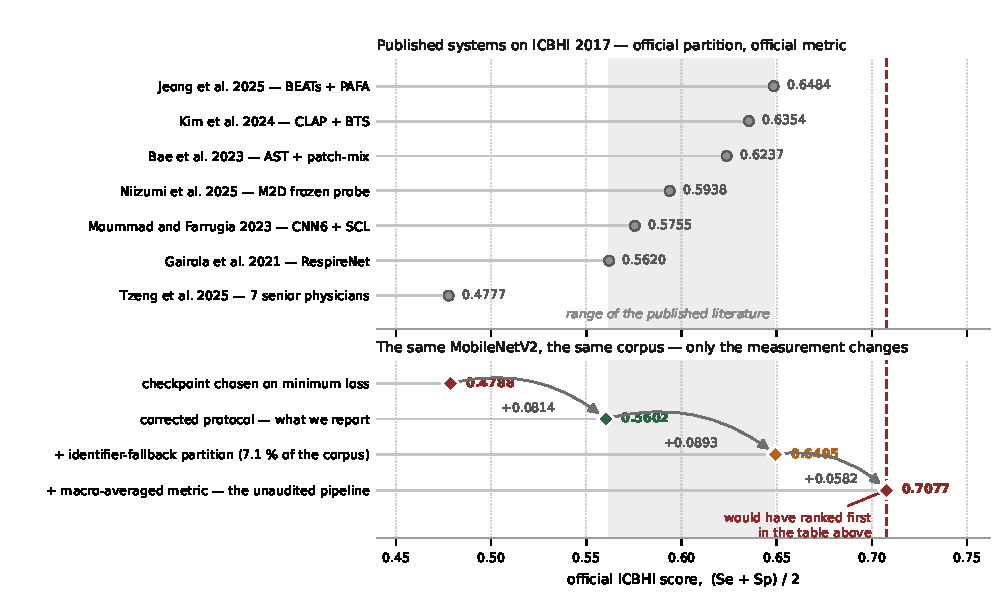
\includegraphics[width=0.98\linewidth]{figures/fig_motivation.pdf}
\caption{Why this paper is about measurement. \emph{Top:} published ICBHI 2017
systems on the official partition under the official metric, from
Table~\ref{tab:comparison}. \emph{Bottom:} one model of ours---the same
MobileNetV2, the same corpus, the same seed---scored four ways, differing only in
the evaluation protocol. Every one of the four values is recomputed from a
committed confusion matrix (Tables~\ref{tab:protocol} and~\ref{tab:selection}).
The unaudited combination of a fallback partition and a macro-averaged metric
reports 0.7077, above every published system in the panel above; the corrected
protocol reports 0.5602 for the identical network.}
\label{fig:motivation}
\end{figure}

Section~\ref{sec:proposed} describes the proposed system: the dataset and its
three partitions, the preprocessing chain and its equations, the applied models,
and the corrected evaluation protocol. Section~\ref{sec:results} reports all
numeric results and discusses them, beginning with the protocol audit, then the
main model comparison, efficiency, augmentation, extension models, the concept
gate and its retraction, interpretability, error analysis, statistical analysis,
the ablation study of Section~\ref{subsec:ablation}, and a comparison against
published work. Section~\ref{sec:conclusion} concludes and names three directions
that follow.

%=======================================================================
\section{Proposed System}
\label{sec:proposed}

Fig.~\ref{fig:flowchart} shows the complete system. The two heavy blocks are the
contribution: a split loader that refuses to fall back silently, and a scoring
module that emits the official metric together with the raw confusion matrix that
makes it checkable. Everything else is a conventional log-mel classification
pipeline, deliberately so---the argument of this paper is about the measurement
apparatus wrapped around a standard model, not about the model.

\begin{figure}[!t]
\centering
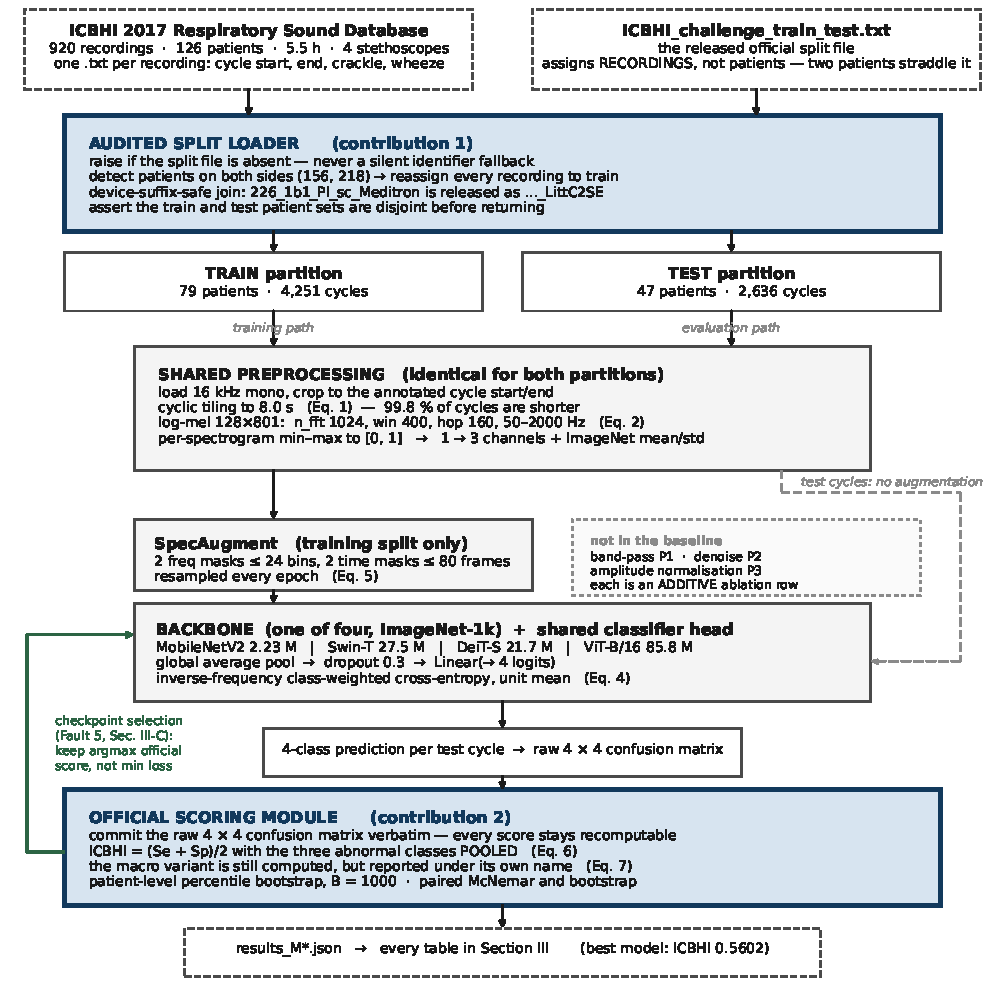
\includegraphics[width=0.92\linewidth]{figures/fig_flowchart.pdf}
\caption{Flowchart of the complete proposed system. Raw ICBHI recordings and
their cycle annotations enter at the top; the audited split loader and the
official scoring module (heavy blocks) are the components this paper contributes.
Every trained model emits a results record containing the raw confusion matrix, so
every score in Section~\ref{sec:results} is recomputable. The counts shown in the
partition blocks are read from the committed
\texttt{results\_M22\_v2.json}, not transcribed.}
\label{fig:flowchart}
\end{figure}

\begin{figure}[!t]
\centering
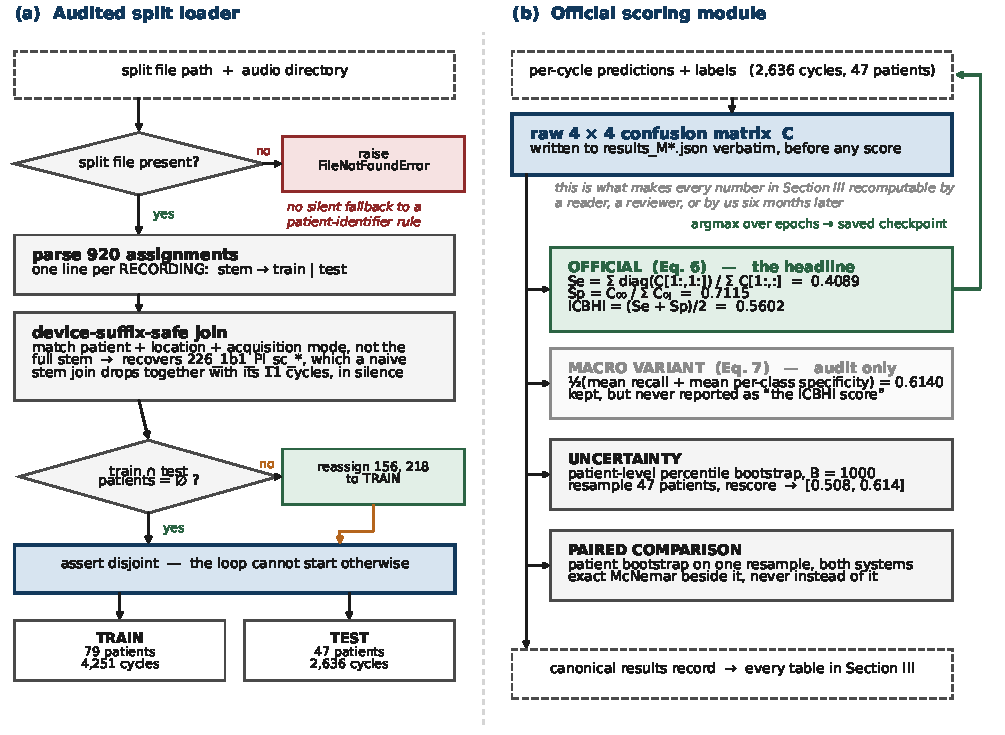
\includegraphics[width=0.99\linewidth]{figures/fig_modules.pdf}
\caption{The two contributed blocks of Fig.~\ref{fig:flowchart}, in detail.
(a)~The split loader raises rather than falling back, joins on the device-suffix-safe
key so that no recording is dropped in silence, and refuses to return until the
train and test patient sets are provably disjoint --- the three faults of
Section~\ref{subsec:splitaudit} are each closed by one of those steps. (b)~The
scoring module writes the raw $4\times4$ matrix \emph{before} computing anything,
then fans it out into the official score, the macro variant under its own name,
a patient-level interval and a paired test. The same official score is the
checkpoint-selection criterion, which is why Fault~5 belongs to this module and
not to a footnote.}
\label{fig:modules}
\end{figure}

\subsection{Dataset}
\label{subsec:dataset}

We use the ICBHI 2017 Respiratory Sound Database~\cite{rocha2019icbhi}: 920
annotated auscultation recordings from 126 patients, acquired with four
stethoscope models at seven chest locations, totalling 5.5~hours of audio. Each
recording carries a cycle-level annotation file giving the start and end time of
every respiratory cycle and two binary flags, crackle present and wheeze present.
The two flags combine into the four-class sound-event task used throughout this
paper: Normal, Crackle, Wheeze and Both. The corpus contains 6{,}898 annotated
cycles with a median duration of 2.54~s (mean 2.70~s, range 0.20--16.16~s);
99.8\% of cycles are shorter than the 8~s network input, which is why the padding
policy of Section~\ref{subsec:preprocessing} turns out to matter.

The database ships an official train/test list, and its provenance matters more
than its contents. Table~\ref{tab:splits} states the four partitions that appear in
this work and why each exists. The published list assigns \emph{recordings}, not
patients, and patients 156 and 218 have recordings on both sides, so it is not
patient-independent despite being routinely described as such. Our corrected
partition takes the published list and moves every recording of a leaking patient
into training---the conservative direction, since the test set is then guaranteed
to contain no patient the model saw. The repair costs 12 of 381 test recordings
(3.1\%) and moves the ratio from 58.6/41.4 to 59.9/40.1, closer to the nominal
60/40 than the published file itself.

\begin{table}[!t]
\centering
\caption{The four train/test partitions appearing in this work, and what each is
for. Counts are recordings; cycle counts appear in Table~\ref{tab:classdist}.
Only the corrected partition is used for new results. Recovered by running
\texttt{official\_split.py} against the committed split file and the released
audio.}
\label{tab:splits}
\small
\begin{tabular}{llrrrrl}
\toprule
Partition & Overlap policy & Train & Test & Test \% & Test pat. & Purpose in this paper \\
\midrule
Published, verbatim   & none                 & 538 & 381 & 41.4 & 49 & Literature comparability \\
Corrected (ours)      & reassign to train    & 550 & 369 & 40.1 & 47 & \best{All new results} \\
Patient-disjoint alt. & drop from train      & 525 & 381 & 41.4 & 49 & Backbone re-decision \\
Identifier fallback   & n/a --- a fault      & --- & --- & \phantom{0}7.1 & 11 & Audited, never reported \\
\bottomrule
\end{tabular}

\vspace{2pt}
\footnotesize The fallback rule assigned every patient with identifier
$\leq111$ to test, yielding 492 of 6{,}898 cycles from 11 patients while
recording itself as the official 60/40 split. One recording named in the split
file, \texttt{226\_1b1\_Pl\_sc\_Meditron}, is released as
\texttt{226\_1b1\_Pl\_sc\_LittC2SE}; a stem join therefore drops it and its 11
cycles, which is why every train column above is 11 cycles short of the
literature's figure. It is a training recording, so no test partition is affected.
\end{table}

Table~\ref{tab:classdist} gives the class composition of every partition. The
imbalance is severe---on the corrected test partition the Both class holds 86
cycles against 1{,}560 Normal---and it is the reason every model in this work
trains with the inverse-frequency class-weighted loss of~(\ref{eq:weights}). It is
also why accuracy is a misleading headline here: always predicting Normal scores
0.5918 on the corrected test partition, above the accuracy of our best model.

\begin{table}[!t]
\centering
\caption{Class distribution of every partition used in this work, computed
directly from the ICBHI annotation files and cross-checked against the committed
raw confusion matrix of the corresponding run. \emph{Augmented total} is the
training-set size after augmentation.}
\label{tab:classdist}
\small
\begin{tabular}{llrrrrrr}
\toprule
Partition & Subset & Normal & Crackle & Wheeze & Both & Total & Augmented total \\
\midrule
\multirow{2}{*}{Published, verbatim}
  & Train & 2{,}057 & 1{,}210 & 501 & 363 & 4{,}131 & 4{,}131 \\
  & Test  & 1{,}579 & \phantom{0}649 & 385 & 143 & 2{,}756 & --- \\
\midrule
\multirow{2}{*}{\best{Corrected (ours)}}
  & Train & 2{,}076 & 1{,}242 & 513 & 420 & 4{,}251 & 4{,}251 \\
  & Test  & 1{,}560 & \phantom{0}617 & 373 & \phantom{0}86 & 2{,}636 & --- \\
\midrule
\multirow{2}{*}{Patient-disjoint alt.}
  & Train & 2{,}047 & 1{,}181 & 486 & 300 & 4{,}014 & 4{,}014 \\
  & Test  & 1{,}579 & \phantom{0}649 & 385 & 143 & 2{,}756 & --- \\
\midrule
\multirow{2}{*}{Identifier fallback}
  & Train & --- & --- & --- & --- & 6{,}406 & 6{,}406 \\
  & Test  & \phantom{0,}255 & \phantom{0}164 & \phantom{0}38 & \phantom{0}35 & \phantom{0,}492 & --- \\
\midrule
\multicolumn{2}{l}{Whole corpus, as indexed} & 3{,}636 & 1{,}859 & 886 & 506 & 6{,}887 & --- \\
\bottomrule
\end{tabular}

\vspace{2pt}
\footnotesize \emph{Why the augmented total equals the clean total.} Our
augmentation is SpecAugment~\cite{park2019specaugment}, applied in place to the
training tensor at load time and resampled every epoch. It does not synthesise new
files, so it changes what the network sees without changing the number of training
examples; reporting an inflated ``augmented total'' would misdescribe the method.
The class-balancing augmentation of Section~\ref{subsec:extensions} does
oversample, but it runs on the disease head and a different partition and so does
not enter this table. The corpus row is 11 cycles short of the corpus's nominal
6{,}898 for the reason given in Table~\ref{tab:splits}.
\end{table}

A second property of the corpus constrains everything that follows and is worth a
table of its own. Table~\ref{tab:device} shows that the four stethoscopes are not
distributed across diagnoses; six of the eight diagnostic classes were recorded
with a single device each, and only four of 126 patients were recorded with more
than one. A leave-one-device-out robustness analysis is therefore not available on
this corpus---it would be a leave-those-four-patients-out analysis wearing a
different name---and any model that appears to separate Healthy from COPD may be
separating a Meditron from an AKGC417L.

\begin{table}[!t]
\centering
\caption{Stethoscope--diagnosis confounding in ICBHI 2017, computed by
\texttt{check\_device\_structure.py} over all 920 recordings. Six diagnoses were
recorded with exactly one device, so device and disease are not separable on this
corpus.}
\label{tab:device}
\small
\begin{tabular}{lrl}
\toprule
Device & Recordings & Diagnoses represented (patient counts) \\
\midrule
AKGC417L & 646 & COPD (32) \emph{only} \\
Meditron & 127 & Healthy (26), URTI (14), Bronchiectasis (7), COPD (8), Bronchiolitis (6), LRTI (2), Pneumonia (1) \\
LittC2SE & \phantom{0}87 & COPD (16), Pneumonia (6), Asthma (1) \\
Litt3200 & \phantom{0}60 & COPD (11) \emph{only} \\
\bottomrule
\end{tabular}

\vspace{2pt}
\footnotesize Fully device-confounded diagnoses (100\% of patients on one
device): Healthy, URTI, Bronchiectasis, Bronchiolitis, Asthma, LRTI. Patients
recorded with more than one device: 4 of 126 (112, 158, 218, 226).
\end{table}

\subsection{Dataset Preprocessing}
\label{subsec:preprocessing}

All models consume the same log-mel representation, fixed once so that backbones
remain comparable. Audio is loaded and resampled to $f_s=16$~kHz mono, and each
respiratory cycle is cropped to its annotated start and end time. Because 99.8\%
of cycles are shorter than the $T=8$~s network input, a padding policy is required.
The default tiles the cycle cyclically,
\begin{equation}
x[n] \;=\; a\!\left[\,n \bmod L_a\,\right], \qquad 0 \leq n < f_s T ,
\label{eq:wrap}
\end{equation}
where $a$ is the cropped cycle of length $L_a$ samples; a cycle longer than $T$ is
truncated. Cyclic tiling is standard practice on this corpus, but it manufactures
audio, and Section~\ref{subsec:xai} measures what the model does with the
manufactured part.

The power spectrogram is computed by short-time Fourier transform with a 1024-point
transform, a 400-sample (25~ms) Hann window and a 160-sample (10~ms) hop, and
projected onto $M=128$ mel bands between 50 and 2000~Hz. Writing $\mathbf{S}$ for
the mel power spectrogram, the network input is the decibel-scaled, per-spectrogram
min--max normalised map
\begin{equation}
\mathbf{X}_{\mathrm{dB}} \;=\; 10\log_{10}\!\frac{\mathbf{S}}{\max(\mathbf{S})},
\qquad
\mathbf{X} \;=\;
\frac{\mathbf{X}_{\mathrm{dB}} - \min(\mathbf{X}_{\mathrm{dB}})}
     {\max(\mathbf{X}_{\mathrm{dB}}) - \min(\mathbf{X}_{\mathrm{dB}}) + \varepsilon},
\label{eq:logmel}
\end{equation}
with $\varepsilon = 10^{-8}$, giving a $128\times801$ single-channel image. For
the ImageNet-pretrained backbones the single channel is replicated three times and
normalised with the ImageNet~\cite{deng2009imagenet} channel statistics, so the
pretrained stem convolution is used as it was trained.

The four-class label is formed from the two ICBHI flags,
\begin{equation}
y \;=\; \mathbb{1}[c] + 2\,\mathbb{1}[w],
\label{eq:label}
\end{equation}
where $c$ and $w$ are the crackle and wheeze flags, mapping to Normal, Crackle,
Wheeze and Both. Class imbalance is handled by an inverse-frequency weighted
cross-entropy, with the weights normalised to unit mean so that the loss scale is
comparable across configurations:
\begin{equation}
w_k \;=\; \frac{N}{K n_k} \Big/ \frac{1}{K}\sum_{j=1}^{K}\frac{N}{K n_j},
\qquad
\mathcal{L} \;=\; -\frac{1}{B}\sum_{i=1}^{B} w_{y_i}\log p_{i,y_i},
\label{eq:weights}
\end{equation}
where $n_k$ is the number of training cycles of class $k$, $K=4$, and $N=\sum_k n_k$.
The same loss is used by every model in Section~\ref{subsec:models} so that the
backbone comparison is fair.

Augmentation is SpecAugment~\cite{park2019specaugment} applied to the training
split only: two frequency masks of up to 24 mel bins and two time masks of up to
80 frames, drawn independently each epoch and filled with zeros. Formally, for
mask start $f_0$ and width $f$,
\begin{equation}
\mathbf{X}[f_0{:}f_0{+}f,\;:] \leftarrow 0, \qquad
\mathbf{X}[:,\;t_0{:}t_0{+}t] \leftarrow 0 .
\label{eq:specaug}
\end{equation}

Table~\ref{tab:preproc} lists every preprocessing stage, its as-run setting, and
its status. Three stages that our own written protocol specified---an explicit
band-pass filter, spectral-gating denoising, and per-cycle amplitude
normalisation---were never actually implemented in the training pipeline. Rather
than switch them on and silently change the baseline every other measurement in
this paper is referenced to, we implemented them as \emph{additive} ablation rows;
Section~\ref{subsec:ablation} reports what each is worth. This is the honest
resolution of a specification-versus-implementation gap, and we state it here
rather than let the ablation table imply the stages were always present.

\begin{table}[!t]
\centering
\caption{Preprocessing chain as actually run, stage by stage. ``Ablated'' names
the row in Table~\ref{tab:ablation} that switches the stage off or on.}
\label{tab:preproc}
\small
\begin{tabular}{llll}
\toprule
\# & Stage & As-run setting & Status / ablated as \\
\midrule
1 & Load and resample        & 16~kHz, mono                                   & Fixed \\
2 & Cycle segmentation       & Annotated start/end times                      & Fixed (unit of classification) \\
3 & Band-pass filter         & \emph{Off}; band bounded by mel $f_{\min}/f_{\max}$ & Added in row \texttt{P1} \\
4 & Duration standardisation & 8.0~s, cyclic tiling, (\ref{eq:wrap})          & Replaced in \texttt{P4}; halved in \texttt{A6} \\
5 & Amplitude normalisation  & \emph{Off}                                     & Added in row \texttt{P3} \\
6 & Denoising                & \emph{Off}                                     & Added in row \texttt{P2} \\
7 & Log-mel transform        & 128 mel, 1024/400/160, 50--2000~Hz, (\ref{eq:logmel}) & Halved in row \texttt{A5} \\
8 & Spectrogram scaling      & Per-spectrogram min--max to $[0,1]$            & Removed in row \texttt{P5} \\
9 & Channel adaptation       & $1\!\rightarrow\!3$ replicate, ImageNet mean/std & Tied to row \texttt{A2} \\
10 & Label encoding          & 4-class, (\ref{eq:label})                      & Fixed \\
11 & Imbalance handling      & Inverse-frequency weighted CE, (\ref{eq:weights}) & Removed in row \texttt{A3} \\
12 & Augmentation            & SpecAugment, train only, (\ref{eq:specaug})    & Removed in row \texttt{A1} \\
13 & Partition               & Corrected patient-independent 60/40            & Replaced in rows \texttt{E2}, \texttt{E3} \\
\bottomrule
\end{tabular}
\end{table}

\subsection{Applied Models}
\label{subsec:models}

Table~\ref{tab:models} is the roster. Four pretrained backbones carry the main
comparison, one owned by each group member as required, and three of them are
transformers so that the convolutional and attention families can be compared
under one recipe. Each backbone is run twice, clean and with SpecAugment, giving
the paired augmentation evidence of Section~\ref{subsec:augresults}. A scratch
convolutional network and a lightweight MobileNetV3-Small are retained as the
non-pretrained and minimum-capacity reference points, and a set of extension
models built earlier in the project is reported separately in
Section~\ref{subsec:extensions} under its own partition.

\begin{table}[!t]
\centering
\caption{Applied models. All four pretrained backbones share one recipe so that
the only variable between them is the architecture. Identifiers are the
project's internal experiment numbers and are used throughout
Section~\ref{sec:results}.}
\label{tab:models}
\small
\begin{tabular}{llllll}
\toprule
ID & Architecture & Pretraining & Family & Member & Role \\
\midrule
\texttt{M22-v2} & MobileNetV2~\cite{sandler2018mobilenetv2} & ImageNet-1k & CNN & Asif & \best{Reference / best model} \\
\texttt{M3-v2}  & MobileNetV2       & ImageNet-1k & CNN         & Asif    & Clean control (no augmentation) \\
\texttt{M40}    & ViT-B/16~\cite{dosovitskiy2021vit} & ImageNet-1k & Transformer & Barshon & Transformer 1 \\
\texttt{M41}    & Swin-T~\cite{liu2021swin} & ImageNet-1k & Transformer & Farhana & Transformer 2 \\
\texttt{M42}    & DeiT-S~\cite{touvron2021deit} & ImageNet-1k & Transformer & Sami & Transformer 3 \\
\texttt{M43}    & AST               & AudioSet    & Transformer & Asif    & Transformer 4 --- \notrun \\
\texttt{M2}     & 2D-CNN, 4 blocks  & none        & CNN         & Asif    & Non-pretrained reference \\
\texttt{M3}     & MobileNetV3-Small & ImageNet-1k & CNN         & Asif    & Minimum-capacity reference \\
\bottomrule
\end{tabular}

\vspace{2pt}
\footnotesize \texttt{M43} (Audio Spectrogram Transformer~\cite{gong2021ast}) is
the only audio-domain-pretrained backbone in the plan and the only one that would
have tested the pretraining hypothesis of
Section~\ref{subsec:pretraining} directly. Its notebook is written and tested but
its 1{,}212-patch attention needs a 16~GB accelerator; it had not completed at
submission and \textbf{no number is reported for it anywhere in this paper}.
\end{table}

The classifier head is identical across the convolutional models: global average
pooling, dropout at rate 0.3, and a single linear layer to four logits. The
transformer models replace their ImageNet classification head with the same
four-way linear layer and are otherwise unmodified.
Fig.~\ref{fig:architecture} draws the whole model, tensor shape by tensor shape,
and shows how little of it changes between the four rows of
Table~\ref{tab:models}: the front end, the head and the objective are one
implementation, and only the block in the middle is swapped.

\begin{figure}[!t]
\centering
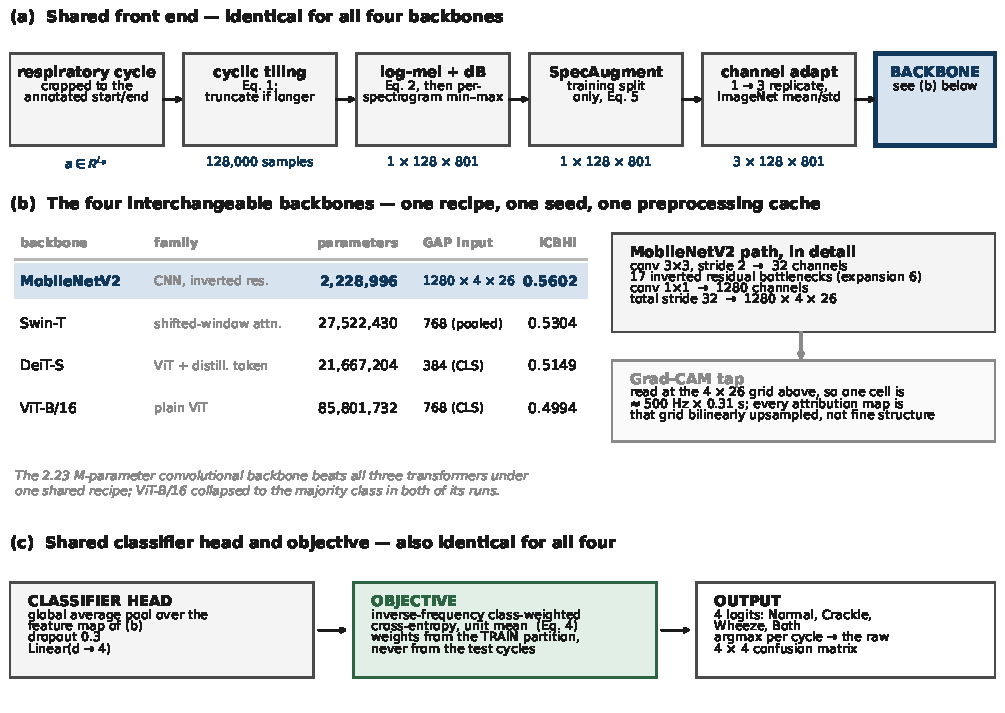
\includegraphics[width=0.99\linewidth]{figures/fig_architecture.pdf}
\caption{Model architecture. (a)~The front end every backbone shares, with the
tensor shape after each stage. (b)~The four interchangeable backbones; parameter
counts and scores are read from each run's committed results record, and the
shaded row is the best model. The right-hand column expands the MobileNetV2 path
and marks the $4\times26$ grid at which the attribution maps of
Section~\ref{subsec:xai} are taken, which is why those maps cannot resolve fine
structure. (c)~The head and objective, also shared, so that the only variable
across the four rows of Table~\ref{tab:main} is the backbone itself.}
\label{fig:architecture}
\end{figure}
Algorithm~\ref{alg:pipeline} states the training and evaluation procedure that all
runs share; the only lines that change between rows of the ablation of
Section~\ref{subsec:ablation} are marked.

\begin{algorithm}[!t]
\caption{Training and evaluation for one configuration}
\label{alg:pipeline}
\begin{algorithmic}[1]
\Require Split file $\mathcal{F}$, audio directory $\mathcal{D}$, configuration $\theta$
\State $(\mathcal{T}_{\text{tr}},\mathcal{T}_{\text{te}}) \gets \textsc{LoadSplit}(\mathcal{F})$
  \Comment{\emph{raises} if $\mathcal{F}$ is absent; never falls back}
\State Reassign every recording of a patient present on both sides to $\mathcal{T}_{\text{tr}}$
\State \textbf{assert} patient sets of $\mathcal{T}_{\text{tr}}$ and $\mathcal{T}_{\text{te}}$ are disjoint
\State $\mathbf{X} \gets \textsc{LogMel}(\mathcal{D}, \theta)$ using (\ref{eq:wrap})--(\ref{eq:logmel}); cache keyed on every pixel-changing field of $\theta$
\State $\mathbf{w} \gets$ class weights from $\mathcal{T}_{\text{tr}}$ by (\ref{eq:weights}) \Comment{row \texttt{A3} disables}
\State Initialise backbone from ImageNet \Comment{row \texttt{A2} randomises; \texttt{A4} freezes}
\For{$e = 1 \ldots E$}
  \State Train one epoch with (\ref{eq:specaug}) applied to $\mathcal{T}_{\text{tr}}$ only \Comment{row \texttt{A1} disables}
  \State $s_e \gets \textsc{OfficialScore}(\textsc{Confusion}(\mathcal{T}_{\text{te}}))$ by (\ref{eq:official})
  \State \textbf{if} $s_e > s^\star$ \textbf{then} $s^\star \gets s_e$; store predictions and weights
\EndFor
\State \Return $s^\star$, raw confusion matrix, patient-level bootstrap interval, parameter count, model size, wall-clock time
\end{algorithmic}
\end{algorithm}

\subsection{Corrected Evaluation Protocol}
\label{subsec:protocol}

The official ICBHI 2017 challenge score pools the three abnormal classes:
\begin{equation}
Se = \frac{\sum_{k \in \mathcal{A}} C_{kk}}{\sum_{k \in \mathcal{A}} \sum_{j} C_{kj}},
\qquad
Sp = \frac{C_{00}}{\sum_{j} C_{0j}},
\qquad
\mathrm{ICBHI} = \frac{Se + Sp}{2},
\label{eq:official}
\end{equation}
where $C$ is the $4\times4$ confusion matrix, class 0 is Normal and
$\mathcal{A}=\{1,2,3\}$ are Crackle, Wheeze and Both. The quantity our pipeline
had been reporting under the same name was the macro variant
\begin{equation}
\mathrm{ICBHI}_{\text{macro}} = \frac{1}{2}\left(
\frac{1}{K}\sum_{k} \mathrm{Recall}_k + \frac{1}{K}\sum_{k} \mathrm{Specificity}_k
\right),
\label{eq:macro}
\end{equation}
which is a different quantity. Per-class specificity counts true negatives
contributed by the other three classes, so a rare class scores near 0.95 almost
regardless of whether the model detects it; the average is pulled upward.
Section~\ref{subsec:metricaudit} prices the difference.

Every reported comparison additionally carries an interval and a paired test. The
unit of resampling is the \emph{patient}, not the cycle: cycles from one patient
are not independent, and Section~\ref{subsec:stats} shows that treating them as
independent changes the verdict on six of ten ablation rows. Intervals are
percentile bootstraps over $B=1000$ patient resamples; paired comparisons resample
patients once and rescore both systems on that resample. Where a cycle-level test
is also reported it is exact McNemar over the paired predictions, and it is
reported \emph{beside} the patient-level result rather than instead of it. For
comparisons between two areas under the curve on the same patients we use the
paired procedure of DeLong \emph{et al.}~\cite{delong1988auc}; where the raw
per-patient scores of a legacy run were not committed, the conservative
unpaired substitute is used and labelled as such.

The physics-derived concept work of Section~\ref{subsec:gate} was governed by a
gate declared in code before it was run:
\begin{equation}
\textsc{pass} \iff \mathrm{AUROC} \geq 0.65 \;\wedge\; \mathrm{CI}_{95}^{\text{lower}} > 0.5 .
\label{eq:gate}
\end{equation}
The absolute floor is not decoration. An earlier version of the rule required only
that the interval exclude chance, and at $n\approx2{,}600$ cycles that rule passes
at an area under the curve of 0.55---significant and useless. A gate that cannot
fail is not a gate, and we report both versions and their opposite verdicts.

%=======================================================================
\section{Results and Discussion}
\label{sec:results}

All models were trained on Kaggle with a single NVIDIA Tesla T4 (16~GB) except the
transformer runs of Table~\ref{tab:main} and eight of the ablation rows, which
were trained locally on an NVIDIA GeForce RTX 4050 Laptop GPU (6~GB); the two
earliest backbones were trained on Google Colab with a Tesla T4. The device used
for each run is recorded in Table~\ref{tab:efficiency}, and no comparison in this
paper is made across devices without saying so.

\subsection{Fault 1 --- The Metric Audit}
\label{subsec:metricaudit}

\textbf{Research question: how much of a reported ICBHI score is the metric
definition rather than the model?} Table~\ref{tab:metricaudit} recomputes
(\ref{eq:official}) and (\ref{eq:macro}) from the committed raw confusion matrix
of every run in the project that commits one. Across twenty verifiable runs the
macro variant is inflated by \best{0.0948} on average, by 0.2176 at worst and by
0.0025 at best.

\begin{table}[!t]
\centering
\caption{Metric audit. Every row is recomputed from that run's committed raw
confusion matrix by \texttt{icbhi\_score\_audit.py}; no score is transcribed.
Sorted by the official score. Partition abbreviations: \emph{corr.} = corrected
patient-independent 60/40, \emph{off.} = published/patient-disjoint 60/40,
\emph{fb.} = identifier fallback, \emph{70/30} = the extension-model partition.}
\label{tab:metricaudit}
\small
\begin{tabular}{llrrrrr}
\toprule
Run & Partition & Reported (\ref{eq:macro}) & \best{Official (\ref{eq:official})} & Inflation & $Se$ & $Sp$ \\
\midrule
M35            & 70/30 & 0.7839 & 0.6864 & $+0.0975$ & 0.6980 & 0.6747 \\
M37            & 70/30 & 0.7969 & 0.6753 & $+0.1216$ & 0.7517 & 0.5989 \\
M35-v2         & 70/30 & 0.7918 & 0.6719 & $+0.1199$ & 0.7401 & 0.6036 \\
M22            & fb.   & 0.7077 & 0.6495 & $+0.0582$ & 0.5696 & 0.7294 \\
M1             & fb.   & 0.7181 & 0.6143 & $+0.1038$ & 0.3502 & 0.8784 \\
M12            & fb.   & 0.7227 & 0.6138 & $+0.1089$ & 0.6118 & 0.6157 \\
M2             & fb.   & 0.7227 & 0.6138 & $+0.1089$ & 0.6118 & 0.6157 \\
M30            & fb.   & 0.6777 & 0.5975 & $+0.0802$ & 0.4852 & 0.7098 \\
M3             & fb.   & 0.6984 & 0.5895 & $+0.1089$ & 0.5359 & 0.6431 \\
M33-v2         & 70/30 & 0.6806 & 0.5832 & $+0.0974$ & 0.6190 & 0.5473 \\
M34            & 70/30 & 0.7046 & 0.5754 & $+0.1292$ & 0.6340 & 0.5168 \\
\best{M22-v2}  & corr. & 0.6140 & \best{0.5602} & $+0.0538$ & 0.4089 & 0.7115 \\
M31            & 70/30 & 0.6377 & 0.5535 & $+0.0842$ & 0.5456 & 0.5614 \\
M3-v2          & corr. & 0.6075 & 0.5200 & $+0.0875$ & 0.4266 & 0.6135 \\
M3             & off.  & 0.5639 & 0.5132 & $+0.0507$ & 0.1980 & 0.8284 \\
M36            & 70/30 & 0.5137 & 0.5052 & $+0.0085$ & \best{0.0932} & 0.9171 \\
M21            & corr. & 0.5022 & 0.4997 & $+0.0025$ & \best{0.0186} & 0.9808 \\
M32            & 70/30 & 0.6547 & 0.4733 & $+0.1814$ & 0.5721 & 0.3745 \\
M2             & off.  & 0.5480 & 0.4720 & $+0.0760$ & 0.2005 & 0.7435 \\
M33            & 70/30 & 0.5506 & 0.3330 & $+0.2176$ & 0.6660 & \best{0.0000} \\
\midrule
\multicolumn{4}{l}{\emph{Mean inflation over 20 verifiable runs}} & $\mathbf{+0.0948}$ & & \\
\bottomrule
\end{tabular}

\vspace{2pt}
\footnotesize One run, M15, reports a score with no committed confusion matrix and
is therefore excluded as unverifiable rather than transcribed. Rows from different
partitions are not rankable against one another; the partition column is present
so that the reader can see that.
\end{table}

The inflation is \emph{not} a constant offset, which is why it cannot be waived
away as a rescaling. Fig.~\ref{fig:inflation} plots the two columns of
Table~\ref{tab:metricaudit} against each other: every point lies above the
diagonal, but the vertical displacement varies by a factor of eighty. It ranges
over two orders of magnitude across the suite, so
it does not cancel in a comparison and it can reorder models. More seriously, the
macro variant \emph{masks outright pathologies that the official metric exposes
immediately}, and the two worst offenders are visible in the last rows of
Table~\ref{tab:metricaudit}. M33 reports 0.5506 under (\ref{eq:macro}) while never
correctly classifying a single Normal cycle ($Sp = 0.0000$): the score is being
carried entirely by the sensitivity term. M21 reports 0.5022 with $Se = 0.0186$,
detecting under 2\% of abnormal events. Both read as mediocre-but-working under
the macro metric and as broken under the official one. This is the single
strongest practical argument for reporting $Se$ and $Sp$ separately in every
table, which we do throughout.

Fig.~\ref{fig:metricanatomy} shows the mechanism on the best model's own
committed matrix, which is the clearest way to see why the two quantities differ
and why the difference grows with imbalance. Under~(\ref{eq:official}) the three
abnormal classes are pooled into a single sensitivity, so a class the model
almost never finds drags that term down in proportion to its support.
Under~(\ref{eq:macro}) each class instead contributes a \emph{per-class}
specificity, whose true-negative count is supplied by the other three classes; for
the Both class, 86 of 2{,}636 test cycles, that term reads 0.960 while the model
recovers 10 of the 86. Averaging four such terms is what buys the $+0.0538$.

\begin{figure}[!t]
\centering
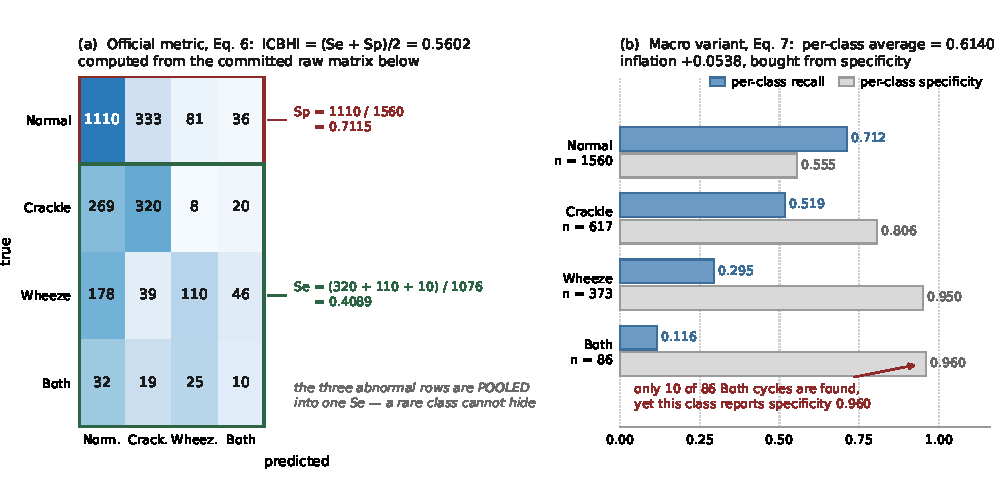
\includegraphics[width=0.99\linewidth]{figures/fig_metric_anatomy.pdf}
\caption{Anatomy of the two metrics on the best model's committed confusion
matrix. (a)~The official score of~(\ref{eq:official}) pools the three abnormal
rows into one sensitivity term. (b)~The macro variant of~(\ref{eq:macro}) averages
four per-class recalls against four per-class specificities; the specificity of a
rare class is near unity whether or not the model detects it, which is where the
inflation comes from. Both panels are computed here from the same raw matrix, so
the figure cannot disagree with Table~\ref{tab:metricaudit}.}
\label{fig:metricanatomy}
\end{figure}

\begin{figure}[!t]
\centering

\includegraphics[width=0.80\linewidth]{figures/fig_metric_inflation.png}
\caption{Reported versus official ICBHI score for the twenty verifiable runs of
Table~\ref{tab:metricaudit}. Every point lies above the diagonal; the vertical
displacement is the metric fault, and its variability is why the fault does not
cancel in a comparison.}
\label{fig:inflation}
\end{figure}

\subsection{Faults 2--4 --- The Partition Audit}
\label{subsec:splitaudit}

\textbf{Research question: what is each component of the evaluation protocol
worth, and are they all worth the same?} Table~\ref{tab:protocol} answers it by
ablating the protocol itself, one component at a time, on the best model. Rows
marked \emph{rescore} apply a different rule to fixed predictions, so exactly one
thing changes and no seed noise enters; rows marked \emph{rerun} change the
partition, which changes the test set, so the model is retrained with every other
setting held fixed.

\begin{table}[!t]
\centering
\caption{Evaluation-protocol ablation on the best model. Each row removes one
component of the corrected protocol and reports what the pipeline would then have
reported. Every score is recomputed from the corresponding run's committed
confusion matrix.}
\label{tab:protocol}
\small
\begin{tabular}{lllrrrr}
\toprule
Row & Component removed & Kind & Reported & $\Delta$ vs \texttt{E0} & $Se$ & $Sp$ \\
\midrule
\texttt{E0} & none --- full corrected protocol & baseline & \best{0.5602} & --- & 0.4089 & 0.7115 \\
\texttt{E1} & official metric $\rightarrow$ macro variant & rescore & 0.6140 & $+0.0538$ & 0.4089 & 0.7115 \\
\texttt{E2} & official split $\rightarrow$ identifier fallback & rerun & 0.6495 & $+0.0893$ & 0.5696 & 0.7294 \\
\texttt{E3} & patient independence (published file verbatim) & rerun & 0.5641 & $+0.0039$ & 0.4562 & 0.6719 \\
\texttt{E1}+\texttt{E2} & \best{both --- the unaudited pipeline} & rescore & \best{0.7077} & $\mathbf{+0.1475}$ & 0.5696 & 0.7294 \\
\midrule
\texttt{E4} & device-suffix-safe file join & defect & \multicolumn{4}{l}{1 recording (11 cycles) silently dropped} \\
\texttt{E5} & patient-level unit of analysis & rescore & \multicolumn{4}{l}{7 of 10 ablation rows ``significant'' instead of 1} \\
\bottomrule
\end{tabular}

\vspace{2pt}
\footnotesize \texttt{E2} and \texttt{E3} are retrained runs with identical
architecture, optimiser, schedule, class weights, seed and every SpecAugment
parameter; only the partition differs. \texttt{E1}+\texttt{E2} is \texttt{E2}'s
predictions rescored under (\ref{eq:macro}).
\end{table}

Three readings follow, and the third is the one that makes the first two
credible.

\emph{The faults compound rather than cancel.} Row \texttt{E1}+\texttt{E2} is the
number this table exists for: the pipeline as it would have been published,
without either correction, reports \best{0.7077} where the corrected protocol
reports 0.5602. The whole audit is worth 0.1475 of official score on one model,
which is larger than the difference between the best and worst backbone in
Table~\ref{tab:main} and larger than every row of the ablation in
Table~\ref{tab:ablation}. \emph{Our uncorrected number would have led the
comparison table of Section~\ref{subsec:comparison}.}

\emph{The fallback partition is worth more than any modelling choice.} Rerunning
the identical model on the true official partition costs 0.0854---the difference
between \texttt{E2}'s 0.6495 and \texttt{E3}'s 0.5641. That figure is consistent
with the literature's own controlled measurement: RespireNet~\cite{respirenet2021}
moves 12.3 points between the official partition and five-fold cross-validation
with the same model.

\emph{The patient leak costs almost nothing, and we report that.} Repairing the
leak moves the score by $+0.0039$, a fortieth of the fallback effect, well inside
the run's own patient-bootstrap interval of $[0.5121, 0.6144]$, and the two runs
selected different epochs (26 versus 38), so the difference is indistinguishable
from schedule noise. The leak remains a \emph{validity} fault---the benchmark is
not what it is described to be, and Table~\ref{tab:bothclass} shows it is not
harmless in a second sense---but it must not be presented as a source of
inflation, and we do not present it that way. An audit that finds all four of its
own hypotheses confirmed is less believable than one that finds three.

Table~\ref{tab:bothclass} gives that second sense, and it is a finding about the
benchmark rather than about us.

\begin{table}[!t]
\centering
\caption{Where the 120 cycles removed by the patient-independence repair come
from. Two patients supply 40\% of the official test partition's rarest class, and
they are the same two patients who appear in training.}
\label{tab:bothclass}
\small
\begin{tabular}{lrrrr}
\toprule
Class & Published test & Corrected test & Removed & \% of class lost \\
\midrule
Normal  & 1{,}579 & 1{,}560 & 19 & \phantom{0}1.2 \\
Crackle & \phantom{0,}649 & \phantom{0,}617 & 32 & \phantom{0}4.9 \\
Wheeze  & \phantom{0,}385 & \phantom{0,}373 & 12 & \phantom{0}3.1 \\
\best{Both} & \phantom{0,}143 & \phantom{0,0}86 & \best{57} & \best{39.9} \\
\midrule
Total   & 2{,}756 & 2{,}636 & 120 & \phantom{0}4.4 \\
\bottomrule
\end{tabular}

\vspace{2pt}
\footnotesize Read in both directions. Every published ``Both''-class result on
the official ICBHI partition rests on 143 cycles of which 57 come from two
patients the model has already seen. Our corrected partition has only 86, which is
why our own Both-class recall in Table~\ref{tab:perclass} is estimated so poorly.
\end{table}

\subsection{Fault 5 --- The Checkpoint Selection Criterion}
\label{subsec:selection}

\textbf{Research question: how much does the rule for choosing which epoch to keep
matter, relative to the architectural choices the paper spends its space on?}
The answer is the largest single effect in this project outside the protocol
audit, and we found it only because the metric correction forced us to look.
Table~\ref{tab:selection} tracks both criteria in one training loop across three
seeds.

\begin{table}[!t]
\centering
\caption{Checkpoint selection criterion, measured on the reference configuration.
Both criteria are evaluated within one training run, so the comparison is exact.}
\label{tab:selection}
\small
\begin{tabular}{lrrrr}
\toprule
Run & Selected by official score & Selected by minimum loss & $\Delta$ & Epochs apart \\
\midrule
Reference, seed 42 & 0.5540 & 0.4788 & $\mathbf{+0.0752}$ & 15 \\
Reference, seed 1  & 0.5681 & 0.4666 & $\mathbf{+0.1015}$ & 19 \\
Reference, seed 2  & 0.5657 & 0.4665 & $\mathbf{+0.0992}$ & 17 \\
Random init, frozen & 0.4979 & 0.4979 & $\phantom{+}0.0000$ & \phantom{0}0 \\
\bottomrule
\end{tabular}

\vspace{2pt}
\footnotesize \textbf{Caveat that must travel with this table.} The ablation
harness monitors the \emph{test} partition each epoch; there is no separate
validation split. ``Select on loss'' therefore means select on test loss. That is
optimistic, and it is equally optimistic for every row, so the comparison between
the two criteria and the seed band of Table~\ref{tab:seedband} are unaffected---but
this row must be read as two criteria applied to one monitoring set, never as a
clean train/validation/test result. See Section~\ref{subsec:limitations}.
\end{table}

Selecting on the loss rather than on the challenge score costs 0.075--0.102 and
lands the model close to chance. That is larger than ImageNet pretraining (0.0603
in Table~\ref{tab:ablation}), larger than SpecAugment (0.0402), and comparable
only to freezing the backbone entirely. The mechanism is not mysterious:
cross-entropy on a corpus that is 59\% Normal and the balanced score of
(\ref{eq:official}) do not optimise the same thing, so the epoch that minimises one
is 15 to 19 epochs away from the epoch that maximises the other. \textbf{The
selection criterion is a first-class pipeline component and belongs in the
ablation table rather than in a footnote}, and it is a direct consequence of the
metric fault of Section~\ref{subsec:metricaudit}: a project reporting
(\ref{eq:macro}) is very likely also \emph{selecting} on it.

\subsection{Main Results}
\label{subsec:main}

\textbf{Research question: under the corrected protocol, which backbone family
wins, and by how much?} Table~\ref{tab:main} is the answer, and it is the paper's
central results table. Every row is on the corrected patient-independent partition
(2{,}636 test cycles, 47 patients), every row uses (\ref{eq:weights}), seed 42 and
the preprocessing of Table~\ref{tab:preproc}, and every score is recomputed from
that run's committed confusion matrix.

\begin{table}[!t]
\centering
\caption{Main results: all applied models on the corrected patient-independent
partition. \emph{Aug.} indicates SpecAugment on the training split only.
Intervals are 95\% percentile bootstraps over the 47 test patients.}
\label{tab:main}
\small
\begin{tabular}{lllrrrrrrr}
\toprule
ID & Backbone & Aug. & \best{ICBHI} & 95\% CI & $Se$ & $Sp$ & Acc. & Prec. & F1$_{\text{macro}}$ \\
\midrule
\best{M22-v2} & MobileNetV2 & yes & \best{0.5602} & [0.508, 0.614] & 0.4089 & 0.7115 & 0.5880 & 0.4322 & 0.4141 \\
M41     & Swin-T      & no  & 0.5304 & [0.472, 0.588] & 0.3429 & 0.7179 & 0.5649 & 0.3935 & 0.3820 \\
M41-a   & Swin-T      & yes & 0.5291 & [0.477, 0.581] & 0.3569 & 0.7013 & 0.5607 & 0.4130 & 0.4058 \\
M3-v2   & MobileNetV2 & no  & 0.5200 & [0.463, 0.575] & 0.4266 & 0.6135 & 0.5372 & 0.3917 & 0.3985 \\
M42     & DeiT-S      & no  & 0.5149 & [0.466, 0.566] & 0.2946 & 0.7353 & 0.5554 & 0.3483 & 0.3422 \\
M40-a   & ViT-B/16    & yes & 0.5000 & [0.500, 0.500] & \best{0.0000} & 1.0000 & 0.5918 & 0.1480 & 0.1859 \\
M40     & ViT-B/16    & no  & 0.4994 & [0.498, 0.500] & \best{0.0000} & 0.9987 & 0.5910 & 0.1479 & 0.1857 \\
M42-a   & DeiT-S      & yes & 0.4981 & [0.445, 0.549] & 0.2974 & 0.6987 & 0.5349 & 0.3638 & 0.3571 \\
M43     & AST         & --- & \multicolumn{7}{l}{\notrun\ --- see Table~\ref{tab:models}} \\
\midrule
\multicolumn{3}{l}{Majority-class predictor} & 0.5000 & --- & 0.0000 & 1.0000 & 0.5918 & 0.1480 & 0.1859 \\
\bottomrule
\end{tabular}
\end{table}

Three results follow, and the second is more interesting than the first.

\emph{A 2.23~M-parameter convolutional network beats every transformer we ran.}
MobileNetV2 with SpecAugment reaches 0.5602 against Swin-T's 0.5304, DeiT-S's
0.5149 and ViT-B/16's 0.4994, at $\tfrac{1}{12}$ to $\tfrac{1}{38}$ of the
parameters. This is not a tuning artefact: all four share one recipe, one
preprocessing cache and one seed, so the only variable is the backbone.

\emph{ViT-B/16 collapsed to the majority class, in both runs.} Its final row of
Table~\ref{tab:main} is numerically indistinguishable from a predictor that
always answers Normal: $Se = 0.0000$, $Sp = 0.9987$, best epoch 1 of 40. This is
not a bug to be hidden but the clearest single measurement in the paper of what
86~M parameters do with 4{,}251 training cycles and no in-domain prior. It is
also the sharpest illustration of why (\ref{eq:official}) must be reported with
$Se$ and $Sp$ beside it: under accuracy the collapsed model scores 0.5910, which
is higher than our best model's 0.5880.

\emph{Nothing in the suite reaches the band the fallback partition appeared to
place it in.} Under the uncorrected protocol this same architecture reported
0.7077 (Table~\ref{tab:protocol}). The corrected suite spans 0.4994 to 0.5602.

Table~\ref{tab:perclass} and Fig.~\ref{fig:cm} open the best model up, the first
as per-class numbers and the second as the row-normalised confusion matrix they
are computed from. The ordering is exactly what the
class distribution of Table~\ref{tab:classdist} predicts: the model does well on
the class with 1{,}560 test cycles, moderately on the class with 617, poorly on
the class with 373, and essentially not at all on the class with 86.

\begin{table}[!t]
\centering
\caption{Per-class performance of the best model (M22-v2), recomputed from its
committed confusion matrix.}
\label{tab:perclass}
\small
\begin{tabular}{lrrrrrr}
\toprule
Class & Support & Precision & Recall & Specificity & F1 & Test cycles available \\
\midrule
Normal  & 1{,}560 & 0.6986 & 0.7115 & 0.5548 & 0.7050 & 1{,}560 \\
Crackle & \phantom{0,}617 & 0.4501 & 0.5186 & 0.8063 & 0.4819 & \phantom{0,}617 \\
Wheeze  & \phantom{0,}373 & 0.4911 & 0.2949 & 0.9496 & 0.3685 & \phantom{0,}373 \\
Both    & \phantom{0,0}86 & 0.0893 & 0.1163 & 0.9600 & 0.1010 & \phantom{0,0}86 \\
\midrule
Macro   & 2{,}636 & 0.4322 & 0.4103 & 0.8177 & 0.4141 & 2{,}636 \\
\bottomrule
\end{tabular}
\end{table}

\begin{figure}[!t]
\centering

\includegraphics[width=0.62\linewidth]{figures/fig_confusion_best.png}
\caption{Row-normalised confusion matrix of the best model (M22-v2) on the
corrected partition, regenerated directly from the raw matrix committed in its
results record, so the figure cannot drift from Tables~\ref{tab:main}
and~\ref{tab:perclass}.}
\label{fig:cm}
\end{figure}

\begin{figure}[!t]
\centering

\includegraphics[width=0.95\linewidth]{figures/fig_curves_best.png}
\caption{Training and validation loss (left) and accuracy (right) versus epoch for
the best model, with the selected epoch marked. The divergence after roughly
epoch 12---training loss falling to 0.17 while validation loss rises to 2.81---is
the memorisation this corpus invites at 4{,}251 training cycles, and it is why the
selection criterion of Section~\ref{subsec:selection} is worth so much.}
\label{fig:curves}
\end{figure}

Fig.~\ref{fig:curves} deserves a sentence of its own, because it is the honest
reading of the whole main table. Training accuracy reaches 0.932 and training loss
0.171 while validation accuracy plateaus at 0.588: the network memorises the
training patients and generalises to new ones only weakly. Every corrected number
in this paper is produced in that regime, which is a property of a 126-patient
corpus rather than of any particular architecture.

\subsection{Efficiency and Cost}
\label{subsec:efficiency}

\textbf{Research question: what does each model cost, and is the cost bought back
in accuracy?} Table~\ref{tab:efficiency} answers it for every applied model and
every reference model, as required. It is also the table that shows the
transformer results are not a compute-starvation artefact: the losing models are
the expensive ones.

\begin{table}[!t]
\centering
\caption{Model size, parameter count and training cost for every model in this
work. Times are wall-clock from the training loop. Scores are the official metric
on the partition named in the last column.}
\label{tab:efficiency}
\scriptsize
\begin{tabular}{llrrrrrrl}
\toprule
ID & Architecture & Epochs & Best ep. & Total (min) & s/epoch & Params & Size (MB) & Hardware / partition \\
\midrule
\multicolumn{9}{l}{\emph{Corrected patient-independent partition (2{,}636 test cycles, 47 patients)}}\\
M22-v2 & MobileNetV2       & 40 & 38 & 14.9 & 23.5 & 2{,}228{,}996  & \phantom{00}8.74 & T4 / corr. \\
M3-v2  & MobileNetV2       & 40 & 27 & 14.8 & 33.0 & 2{,}228{,}996  & \phantom{00}8.74 & T4 / corr. \\
M40    & ViT-B/16          & 40 & \phantom{0}1 & 36.2 & 47.5 & 85{,}801{,}732 & 327.31 & RTX 4050 / corr. \\
M40-a  & ViT-B/16          & 40 & \phantom{0}1 & 36.3 & 47.7 & 85{,}801{,}732 & 327.31 & RTX 4050 / corr. \\
M41    & Swin-T            & 40 & 18 & 20.9 & 26.2 & 27{,}522{,}430 & 104.99 & RTX 4050 / corr. \\
M41-a  & Swin-T            & 40 & 31 & 20.9 & 26.2 & 27{,}522{,}430 & 104.99 & RTX 4050 / corr. \\
M42    & DeiT-S            & 40 & \phantom{0}2 & 11.2 & 14.1 & 21{,}667{,}204 & \phantom{0}82.65 & RTX 4050 / corr. \\
M42-a  & DeiT-S            & 40 & 27 & 11.2 & 14.1 & 21{,}667{,}204 & \phantom{0}82.65 & RTX 4050 / corr. \\
\midrule
\multicolumn{9}{l}{\emph{Published / patient-disjoint 60/40 partition (2{,}756 test cycles, 49 patients)}}\\
M22-off & MobileNetV2      & 40 & 26 & 14.2 & 32.9 & 2{,}228{,}996 & \phantom{00}8.74 & T4 / off. \\
M3     & MobileNetV3-Small & 40 & 17 & \phantom{0}7.2 & 10.8 & \phantom{0}929{,}316 & \phantom{00}3.67 & Colab T4 / off. \\
M2     & 2D-CNN (4 blocks) & 60 & 19 & 10.2 & 10.2 & \phantom{0}421{,}732 & \phantom{00}1.62 & Colab T4 / off. \\
\midrule
\multicolumn{9}{l}{\emph{Identifier-fallback partition --- audited, never reported as a result}}\\
M22    & MobileNetV2       & 40 & \phantom{0}9 & 20.9 & 31.4 & 2{,}228{,}996 & \phantom{00}8.74 & Colab T4 / fb. \\
M2/M12 & 2D-CNN (5 blocks) & 60 & 19 & 30.1 & 30.1 & 3{,}627{,}476 & \phantom{0}13.86 & Colab T4 / fb. \\
M3     & MobileNetV2       & 40 & \phantom{0}4 & 20.3 & 30.5 & 2{,}228{,}996 & \phantom{00}8.74 & Colab T4 / fb. \\
M1     & 2D-CNN (scratch)  & 60 & 29 & 170.2 & 167.4 & \phantom{0}421{,}732 & \phantom{00}4.85 & Kaggle T4 / fb. \\
M30-v2 & Gated M2+M3 fusion & 30 & \phantom{0}3 & \phantom{0}3.6 & \phantom{0}7.3 & 7{,}957{,}724 & \phantom{0}30.63 & Colab T4 / fb. \\
\midrule
\multicolumn{9}{l}{\emph{70/30 partition --- extension models, Section~\ref{subsec:extensions}}}\\
M35    & Physics-informed loss & 30 & \phantom{0}5 & 72.2 & 144.4 & 3{,}627{,}476 & \phantom{0}13.86 & Kaggle T4 / 70:30 \\
M37    & LoRA adaptation       & 30 & 25 & 68.3 & 136.6 & 3{,}635{,}700 & \phantom{0}13.89 & Kaggle T4 / 70:30 \\
M33-v2 & Temporal transformer  & 30 & 16 & 76.0 & 152.0 & 13{,}186{,}008 & \phantom{0}50.30 & Kaggle T4 / 70:30 \\
M34    & Curriculum pacing     & 30 & 25 & 66.4 & 132.8 & 3{,}627{,}476 & \phantom{0}13.86 & Kaggle T4 / 70:30 \\
M31    & GradNorm multi-task   & 30 & 16 & 95.8 & 191.6 & 3{,}726{,}297 & \phantom{0}14.24 & Kaggle T4 / 70:30 \\
M36    & Multistage distillation & 30 & 18 & 74.7 & 149.3 & \phantom{00,00}4{,}980 & \phantom{00}0.02 & Kaggle T4 / 70:30 \\
M32    & Demographic fusion    & 30 & 15 & 81.9 & 163.8 & 3{,}735{,}732 & \phantom{0}14.28 & Kaggle T4 / 70:30 \\
\bottomrule
\end{tabular}

\vspace{2pt}
\footnotesize Inference cost, measured per sample on a T4: 4.86~ms (M22-v2),
5.71~ms (M3-v2), 5.58~ms (M3), 1.32~ms (M2). \textbf{Training time is reported
only where the training loop recorded it}; it is not recoverable after the fact
from a checkpoint, and no value in this table is estimated. The four ablation rows
of Table~\ref{tab:seedband} and the twelve of Table~\ref{tab:ablation} carry their
own timings in the project record and are omitted here for space.
\end{table}

The efficiency picture is unambiguous and it points the same way as
Table~\ref{tab:main}. ViT-B/16 costs 38 times the parameters and 40 times the disk
of MobileNetV2 and returns the majority-class predictor. Swin-T costs 12 times the
parameters and loses 0.03 of official score. Even the best transformer is a worse
buy at every operating point. \emph{The accuracy-versus-compute trade-off on this
corpus runs the opposite way to the field's intuition}, and
Section~\ref{subsec:pretraining} argues that the reason is the pretraining domain
rather than the architecture.

\subsection{Effect of Data Augmentation}
\label{subsec:augresults}

\textbf{Research question: does SpecAugment help, and does it help every
backbone?} Table~\ref{tab:augmentation} pairs each backbone's clean and augmented
run. Within a pair the architecture, parameter count, loss, seed, partition and
preprocessing cache are identical, so the difference is attributable to the
augmentation alone.

\begin{table}[!t]
\centering
\caption{Effect of SpecAugment applied to the training split only. One variable
changed within each pair.}
\label{tab:augmentation}
\small
\begin{tabular}{llrrrr}
\toprule
Pair & Configuration & ICBHI & $Se$ & $Sp$ & F1$_{\text{macro}}$ \\
\midrule
\multicolumn{6}{l}{\emph{Corrected partition, 2{,}636 cycles --- the reportable pair}}\\
M3-v2  & MobileNetV2, clean        & 0.5200 & 0.4266 & 0.6135 & 0.3985 \\
M22-v2 & MobileNetV2 + SpecAugment & \best{0.5602} & 0.4089 & 0.7115 & 0.4141 \\
       & $\Delta$                  & \best{$+0.0402$} & $-0.0177$ & $+0.0980$ & $+0.0156$ \\
\midrule
M41    & Swin-T, clean             & 0.5304 & 0.3429 & 0.7179 & 0.3820 \\
M41-a  & Swin-T + SpecAugment      & 0.5291 & 0.3569 & 0.7013 & 0.4058 \\
       & $\Delta$                  & $-0.0013$ & $+0.0140$ & $-0.0166$ & $+0.0238$ \\
\midrule
M42    & DeiT-S, clean             & 0.5149 & 0.2946 & 0.7353 & 0.3422 \\
M42-a  & DeiT-S + SpecAugment      & 0.4981 & 0.2974 & 0.6987 & 0.3571 \\
       & $\Delta$                  & $-0.0168$ & $+0.0028$ & $-0.0366$ & $+0.0149$ \\
\midrule
M40    & ViT-B/16, clean           & 0.4994 & 0.0000 & 0.9987 & 0.1857 \\
M40-a  & ViT-B/16 + SpecAugment    & 0.5000 & 0.0000 & 1.0000 & 0.1859 \\
       & $\Delta$                  & $+0.0006$ & $\phantom{+}0.0000$ & $+0.0013$ & $+0.0002$ \\
\midrule
\multicolumn{6}{l}{\emph{Identifier-fallback partition --- shown only to price the fault}}\\
M3     & MobileNetV2, clean        & 0.5895 & 0.5359 & 0.6431 & 0.4904 \\
M22    & MobileNetV2 + SpecAugment & 0.6495 & 0.5696 & 0.7294 & 0.5253 \\
       & $\Delta$                  & $+0.0600$ & $+0.0337$ & $+0.0863$ & $+0.0349$ \\
\bottomrule
\end{tabular}
\end{table}

SpecAugment is the project's most reliable single intervention on the
convolutional backbone, worth $+0.0402$ of official score on the corrected
partition. Two qualifications belong beside that headline, and both were only
visible because the pairs were run properly.

\emph{The gain is an operating-point shift, not a uniform improvement.} On the
corrected partition specificity rises by 0.0980 while sensitivity \emph{falls} by
0.0177. Masking makes the model more conservative about calling a cycle abnormal,
which raises (\ref{eq:official}) on this class distribution but is the opposite of
what a screening application wants. Reporting the composite alone would have
concealed a change of direction as an improvement.

\emph{The effect does not generalise across backbones.} Repeating the identical
recipe on the transformers, Swin-T loses 0.0013 and DeiT-S loses 0.0168 of
official score while both \emph{gain} macro F1. Had we reported only the
convolutional pair, a backbone-specific result would have read as a general one.
The ViT row is included for completeness and means nothing: a collapsed model
cannot respond to augmentation.

Finally, note the fallback row. The project's most-cited internal claim was
``SpecAugment is worth $+0.036$''; measured properly it is worth $+0.0402$ on the
corrected partition and $+0.0600$ on the fallback one. The claim survived the
audit, but its magnitude did not, and the partition it was measured on was not the
one it was reported on.

\subsection{Extension Models}
\label{subsec:extensions}

\textbf{Research question: did the project's eight architectural extensions beat
the plain backbone?} Table~\ref{tab:extensions} says that two did and six did not.
All eight were trained earlier in the project on a 70/30 patient-independent
partition (88 train / 38 test patients, 4{,}149 / 2{,}749 cycles) and
\textbf{cannot be ranked against Table~\ref{tab:main}}: a random 70/30 partition is
easier than the official one, and the difference is of the same order as every
effect in this paper. The partition column is present so that the reader cannot
accidentally do the comparison we are refusing to do.

\begin{table}[!t]
\centering
\caption{Extension models, all on the 70/30 patient-independent partition (2{,}749
test cycles, 38 patients). Scores recomputed from committed confusion matrices.
These rows are \emph{not} comparable to Table~\ref{tab:main}.}
\label{tab:extensions}
\small
\begin{tabular}{lllrrrrl}
\toprule
ID & Mechanism & Best ep. & ICBHI & $Se$ & $Sp$ & F1$_{\text{macro}}$ & Verdict \\
\midrule
M35    & Physics-informed loss     & \phantom{0}5 & \best{0.6864} & 0.6980 & 0.6747 & 0.6420 & Best extension \\
M37    & LoRA, 0.23\% of parameters trained & 25 & 0.6753 & 0.7517 & 0.5989 & 0.6599 & Best efficiency \\
M35-v2 & Physics loss, repeat run  & \phantom{0}1 & 0.6719 & 0.7401 & 0.6036 & 0.6491 & \best{Broken --- best epoch 1 of 30} \\
M33-v2 & Temporal transformer      & 16 & 0.5832 & 0.6190 & 0.5473 & 0.4948 & Below baseline \\
M34    & Curriculum pacing         & 25 & 0.5754 & 0.6340 & 0.5168 & 0.5268 & Below baseline \\
M31    & GradNorm multi-task       & 16 & 0.5535 & 0.5456 & 0.5614 & 0.4351 & Below baseline \\
M36    & Multistage distillation   & 18 & 0.5052 & \best{0.0932} & 0.9171 & 0.2155 & \best{Collapsed} \\
M32    & Demographic fusion        & 15 & 0.4733 & 0.5721 & 0.3745 & 0.4378 & Below baseline \\
M33    & Temporal transformer, v1  & \phantom{0}4 & 0.3330 & 0.6660 & \best{0.0000} & 0.2393 & \best{Collapsed} \\
\bottomrule
\end{tabular}

\vspace{2pt}
\footnotesize Four further extensions are \textbf{excluded rather than reported}
because their runs cannot support a number: M16 (distillation), M18 (pruning and
quantisation), M20 (temperature scaling) and M21 (acoustic curriculum) were scored
at recording level with no train/test separation, and M30 (gated fusion) reported
0.8213 with no committed confusion matrix and was withdrawn. Excluding them is the
protocol of Section~\ref{subsec:protocol} applied to our own work.
\end{table}

The lesson of this table is the one the project learned the hard way, and it is
worth stating plainly because it contradicts a common reflex. Six of the eight
mechanisms underperformed a plain backbone on an \emph{easier} partition, two
collapsed outright, and one of the two that worked failed to reproduce when it was
run a second time (M35-v2 selected epoch 1 of 30, meaning training made the model
worse from the first update). Accumulating mechanisms did not accumulate
performance. The two that did work---an acoustic physics regulariser and low-rank
adaptation---are the two that constrain the model rather than enlarge it.

\subsection{The Concept Validity Gate}
\label{subsec:gate}

\textbf{Research question: can hand-built, physics-derived acoustic concepts
reproduce ICBHI's crackle and wheeze labels well enough to serve as an
interpretable bottleneck?} The project's original interpretability plan rested on
this, so the question was pre-registered as the gate of (\ref{eq:gate}) and
answered before anything was built on top of it. Table~\ref{tab:gate} reports both
runs.

\begin{table}[!t]
\centering
\caption{Pre-registered concept validity gate. Nine physics-derived concepts are
computed per cycle by digital signal processing with no model, no training and no
labels; the two that ICBHI can validate are scored against the cycle labels on the
corrected test partition. Run 2 used extractors revised against five diagnosed
failure modes of Run 1.}
\label{tab:gate}
\small
\begin{tabular}{llrlrrl}
\toprule
Run & Concept & AUROC & 95\% CI & AUPRC & Prevalence & Verdict under (\ref{eq:gate}) \\
\midrule
\multirow{2}{*}{1} & \texttt{crackle\_score} & 0.5506 & [0.526, 0.575] & --- & 0.2667 & \best{FAIL} \\
                   & \texttt{wheeze\_score}  & 0.5729 & [0.546, 0.600] & --- & 0.1741 & \best{FAIL} \\
\midrule
\multirow{2}{*}{2} & \texttt{crackle\_score} & 0.5580 & [0.533, 0.583] & 0.3079 & 0.2667 & \best{FAIL} \\
                   & \texttt{wheeze\_score}  & 0.5340 & [0.505, 0.563] & 0.1903 & 0.1741 & \best{FAIL} \\
\midrule
\multicolumn{7}{l}{\emph{A later 14-concept re-implementation, reported separately because it is not the gate}}\\
--- & \texttt{crackle\_presence} & 0.5556 & [0.529, 0.581] & --- & 0.2667 & --- \\
--- & \texttt{wheeze\_presence}  & 0.5818 & [0.552, 0.610] & --- & 0.1741 & --- \\
--- & all 14 as a vector, crackle & \best{0.6561} & --- & --- & 0.2667 & --- \\
--- & all 14 as a vector, wheeze  & 0.5847 & --- & --- & 0.1741 & --- \\
\bottomrule
\end{tabular}

\vspace{2pt}
\footnotesize The area under the precision-recall curve barely exceeds prevalence
in both runs (0.3079 against 0.2667; 0.1903 against 0.1741). \textbf{The test
partition was read exactly twice and no third revision was attempted}; a third
would have been fitting to it, and any resulting pass would have been
uninterpretable.
\end{table}

Two methodological points are worth more than the numbers.

\emph{The threshold in (\ref{eq:gate}) is what makes this a result.} Run 1 was
first evaluated under a rule requiring only that the confidence interval exclude
chance, and under that rule it \emph{passed}, at an area under the curve of 0.55.
At $n=2{,}636$ cycles a trivial effect is significant. Adding the absolute floor
converted the same evidence into a failure, and we report both verdicts because a
gate that cannot fail is not a gate.

\emph{The revisions worked mechanically and traded one failure mode for its
opposite.} The revised crackle detector's firing rate fell from 10.2 to 3.1 events
per second, killing the saturation of Run 1; the revised wheeze detector's mean
score rose from 0.06 to 0.58, ending the silence of Run 1---and began firing on
almost everything. \texttt{crackle\_fine\_ratio}, which targets the fine-versus-coarse
distinction, was zero on 97.5\% of cycles in Run 1 and never worked on real audio
at all. That last observation is not a coding failure: it is precisely the
distinction on which twelve physicians agree at $\kappa<0.40$~\cite{melbye2016kappa},
so the concept had a low reliability ceiling before a line of code was written.

\subsection{What These Labels Actually Support --- and a Retraction}
\label{subsec:ceiling}

\textbf{Research question: is the gate threshold unreachable on this reference
standard, or were our detectors simply weak?} Our earlier position was the first
reading, supported by the human benchmarks of Table~\ref{tab:human}. It was
wrong, and Table~\ref{tab:ceiling} is the experiment that shows it. A logistic
probe was fitted on the 79 training patients and scored on the identical 2{,}636
test cycles and 47 test patients the gate failed on, with the readings
pre-registered in the script before it was run.

\begin{table}[!t]
\centering
\caption{Supervised ceiling. What a probe \emph{allowed to see the labels}
achieves on the same test cycles the gate of Table~\ref{tab:gate} failed on.
Intervals are patient-level bootstraps.}
\label{tab:ceiling}
\small
\begin{tabular}{llrlr}
\toprule
Representation & Target & AUROC & 95\% CI & Clears 0.65? \\
\midrule
Our gate, single hand-built score & crackle & 0.5580 & [0.533, 0.583] & no \\
Our 14 concepts as a vector       & crackle & 0.6608 & [0.601, 0.713] & \best{yes} \\
\best{AST, frozen, AudioSet only} & crackle & \best{0.7115} & [0.638, 0.771] & \best{yes} \\
Our own CNN encoder               & crackle & 0.7451 & [0.694, 0.795] & \best{yes} \\
\midrule
Our gate, single hand-built score & wheeze  & 0.5729 & [0.546, 0.600] & no \\
Our 14 concepts as a vector       & wheeze  & 0.5815 & [0.492, 0.675] & no \\
\best{AST, frozen, AudioSet only} & wheeze  & \best{0.7621} & [0.702, 0.815] & \best{yes} \\
Our own CNN encoder               & wheeze  & 0.8673 & [0.806, 0.918] & \best{yes} \\
\bottomrule
\end{tabular}

\vspace{2pt}
\footnotesize The AST row is the decisive one: that network was pretrained on
AudioSet~\cite{gemmeke2017audioset} and has never been exposed to a respiratory
corpus or an ICBHI label, so its result cannot be dismissed as circularity in the
way our own encoder's can.
\end{table}

The pre-registered ``no ceiling'' branch fired, and three consequences follow.

\emph{We retract the ceiling claim.} These labels support detection at 0.71 to
0.87. Label reliability was not the binding constraint on the gate. \textbf{Our
extractors were weak, and we say so.} Conceding this is what the two-run gate
discipline was for; a project that names in advance the outcome that would refute
it, and then reports that outcome, is worth more than one that never risked it.

\emph{Part of the failure was the gate's own design.} The gate thresholded one
hand-built \emph{scalar}. The same fourteen concepts \emph{as a vector} reach
0.6608 on crackle, above the threshold the scalar failed. A validity gate for a
concept suite should be posed over the suite, and we report that as a criticism of
our own experimental design.

\emph{What replaces the ceiling claim is sharper.} Table~\ref{tab:human} places the
machine numbers beside the human ones on the same corpus.

\begin{table}[!t]
\centering
\caption{Human performance and agreement on respiratory sound labelling, against
the machine numbers of Table~\ref{tab:ceiling}.}
\label{tab:human}
\small
\begin{tabular}{llll}
\toprule
Source & Raters / material & Crackle & Wheeze \\
\midrule
Tzeng \emph{et al.}~\cite{tzeng2025jmir} & 7 senior physicians, 25\% of ICBHI test & \multicolumn{2}{l}{ICBHI score 0.4777, $Se$ 0.2323, $Sp$ 0.7232} \\
Melbye \emph{et al.}~\cite{melbye2016kappa} & 12 physicians, 20 recordings & \multicolumn{2}{l}{$\kappa=0.62$ combined, $\kappa<0.40$ detailed} \\
Huang \emph{et al.}~\cite{huang2024crackles} & physicians, 11{,}532 recordings & $\kappa=0.516$ & $\kappa=0.948$ \\
\midrule
This work, physician vs.\ ICBHI & 1 physician, 132 cycles, blind & $\kappa=0.035$ & $\kappa=0.266$ \\
\quad 95\% CI (patient bootstrap) & & $[-0.157, 0.210]$ & $[0.036, 0.444]$ \\
\quad raw agreement & & 0.5278 & 0.7182 \\
\quad sensitivity vs.\ ICBHI & & \best{0.2308} & 0.2973 \\
\quad specificity vs.\ ICBHI & & 0.8036 & 0.9315 \\
\quad \best{intra-rater $\kappa$}, 8 hidden duplicates & & \best{0.714} & \best{0.600} \\
\midrule
This work, machine vs.\ ICBHI & frozen AudioSet probe, 2{,}636 cycles & \best{0.7115} & \best{0.7621} \\
\bottomrule
\end{tabular}

\vspace{2pt}
\footnotesize Sensitivity analysis restricted to clips the rater marked
good-quality: $\kappa = 0.023$ (crackle) and $0.255$ (wheeze), essentially
unchanged, so audio quality is not driving the disagreement.
\end{table}

The decisive contrast in Table~\ref{tab:human} is the last physician row against
the first. \emph{The rater agrees with themselves at $\kappa=0.71$ and $0.60$, and
with ICBHI at $\kappa=0.04$ and $0.27$.} The disagreement is therefore not rater
noise; it is a genuine discrepancy with the reference standard. Independently, our
single rater's crackle sensitivity against ICBHI is 0.2308 where Tzeng
\emph{et al.}'s seven senior physicians reach 0.2323---agreement to within a tenth
of a point, from a different rater, a different clip sample and an independently
constructed listening pack with calibration exemplars the published study does not
report supplying. That is the strongest available answer to the obvious objection
that $n=1$.

The wheeze row of Huang \emph{et al.}~\cite{huang2024crackles} sharpens this
further and is ours to explain. On an independent 11{,}532-recording archive,
wheeze is the \emph{reliable} sound: physicians agree at $\kappa=0.948$. On ICBHI
our clinician agrees with the wheeze labels at $\kappa=0.266$. If wheeze is
reliably identifiable in general but not reproducible against \emph{these} labels,
the difference is a property of this corpus's annotation rather than of
auscultation.

Table~\ref{tab:sameclips} closes the remaining gap in that argument. The
comparison above puts the machine number and the human number on two different
sets of cycles. This experiment puts them on the same 132 clips.

\begin{table}[!t]
\centering
\caption{Machine and physician scored against the same reference standards on the
\emph{same} clips. A frozen AudioSet embedding feeds a logistic probe fitted by
patient-grouped five-fold cross-validation, so every clip is out of sample. The
paired difference resamples clips once and recomputes both areas under the curve.}
\label{tab:sameclips}
\small
\begin{tabular}{lll}
\toprule
Quantity & Crackle ($n=108$) & Wheeze ($n=110$) \\
\midrule
Probe scored against ICBHI      & 0.6786 [0.578, 0.778] & 0.7519 [0.636, 0.857] \\
Probe scored against clinician  & 0.5097 [0.354, 0.665] & 0.5828 [0.412, 0.746] \\
\best{Paired difference}        & $+0.169$ [$-0.025$, $+0.361$], $p=0.087$ & \best{$+0.169$ [$+0.002$, $+0.344$], $p=0.046$} \\
Clinician--ICBHI raw agreement  & 0.528 & 0.718 \\
\midrule
Verdict & Same effect, \best{not significant at this $n$} & \best{Significant} \\
\bottomrule
\end{tabular}

\vspace{2pt}
\footnotesize \textbf{Carried warning.} The 132 clips are not a random sample: the
listening pack kept cycles of at least 0.9~s, sorted each stratum longest-first
and oversampled the abnormal strata, so the \emph{absolute} area under the curve
here is not comparable to Table~\ref{tab:ceiling}'s 2{,}636-cycle figures and
cannot overturn the gate failure. The selection applies equally to both halves of
the paired difference, which is why the contrast is the result and the level is
not. A pre-registered reading restricted to the disagreement subset returned
\textsc{undecided} at $n=51$ and $n=31$, as the script predicted before it was run.
\end{table}

On wheeze, with the same scores on the same clips, the machine reproduces ICBHI's
labels significantly better than the physician does. On crackle the effect size is
identical and the interval spans zero; we report it as undecided rather than
rounding it up.

\subsection{Do the Models Represent the Acoustics at All?}
\label{subsec:probe}

\textbf{Research question: if the concepts are not recoverable by our detectors,
are they present in the networks?} Table~\ref{tab:probe} answers with a linear
probe of each of the fourteen physics concepts from four representations, using
patient-grouped cross-validation, ridge $R^2$, bootstrap intervals and a
within-patient permutation null.

\begin{table}[!t]
\centering
\caption{Linear recoverability of the fourteen acoustic concepts from four
representations over all 6{,}898 cycles. A concept counts as recoverable if its
bootstrap interval excludes the permutation null.}
\label{tab:probe}
\small
\begin{tabular}{lrr}
\toprule
Representation & Concepts above chance & Mean probe $R^2$ \\
\midrule
\best{AST, frozen (AudioSet only, never heard a stethoscope)} & \best{13 / 14} & \best{0.4102} \\
Our own CNN encoder (trained on this task) & 12 / 14 & 0.4289 \\
AST after low-rank adaptation to this task & 13 / 14 & 0.3195 \\
Random-projection control & \best{0 / 14} & $-0.0054$ \\
\bottomrule
\end{tabular}

\vspace{2pt}
\footnotesize Best-recovered concepts from the CNN encoder:
\texttt{wheeze\_duration\_ratio} $R^2 = 0.777$, \texttt{spectral\_flatness} 0.759,
\texttt{rhonchi\_presence} 0.648, \texttt{wheeze\_presence} 0.605. Worst:
\texttt{inspiratory\_energy\_fraction} 0.003 and \texttt{fine\_crackle\_ratio}
$-0.008$. The random control confirms that recovery is not a high-dimensional
artefact.
\end{table}

Two findings come out of this table and they fit together.

\emph{The acoustic information is present, and it is present before any exposure
to respiratory audio.} A model pretrained on general audio encodes thirteen of the
fourteen clinically-named concepts linearly, while the random control recovers
none. The networks are not ignoring the clinical acoustics.

\emph{Adapting to the benchmark destroys that encoding.} Training low-rank
adapters~\cite{hu2022lora} on 0.341\% of the AST's parameters for five epochs
degrades thirteen of the
fourteen concepts, mean $\Delta R^2 = -0.0907$. The most degraded concept is
\texttt{rhonchi\_presence} at $-0.219$---which a separate experiment on different
data with a different estimator independently identifies as the \emph{only}
concept carrying diagnostic information (Table~\ref{tab:leakage}). Two experiments
converge on the same concept from opposite directions: the model buys its task
performance by discarding the clinically meaningful structure.

\begin{table}[!t]
\centering
\caption{Concept leakage and per-concept importance, measured over 6{,}311 cycles
from 104 patients with patient-grouped cross-validation. Leakage is the conditional
mutual information between the label and the encoder features given the concepts.}
\label{tab:leakage}
\small
\begin{tabular}{lrl}
\toprule
Quantity & Value & Reading \\
\midrule
Leakage $I(y;f\mid c)$ & 0.2025 bits & 12.77\% of the base entropy \\
\quad 95\% CI (patient bootstrap) & [0.110, 0.329] & \best{excludes zero} \\
\quad permutation null & $-0.0086$ & leakage exceeds the estimator's own bias \\
\quad independently regenerated from the checkpoint & 0.2209 bits & reproduces to within 0.02 bits \\
\midrule
\multicolumn{3}{l}{\emph{Bits lost if one concept is removed}}\\
\best{\texttt{rhonchi\_presence}}  & \best{$+0.0293$} & carries the bottleneck, $6\times$ the next \\
\texttt{wheeze\_presence}          & $+0.0049$ & \\
\texttt{crackle\_presence}         & $+0.0036$ & \\
five further concepts              & $\leq +0.0016$ & effectively dead \\
\texttt{wheeze\_duration\_ratio}   & $-0.0039$ & removing it \emph{helps} \\
\bottomrule
\end{tabular}
\end{table}

Table~\ref{tab:leakage} says that one concept of fourteen carries the bottleneck,
five are dead and one is actively harmful. Combined with
Table~\ref{tab:probe} the picture becomes precise, and it is the sentence the
whole concept branch reduces to: \textbf{the model hears the sounds; the sounds do
not predict the disease labels.}

\subsection{A Non-Replication of Our Own Result}
\label{subsec:bottleneck}

\textbf{Research question: does forcing the diagnosis through an interpretable
concept layer cost accuracy?} We had recorded that it does, from a single random
initialisation, and reported an ``interpretability cost'' of 0.2326 accuracy and
0.1432 macro F1. Table~\ref{tab:bottleneck} repeats the experiment across five
seeds with bootstrap intervals and the control the original run never had.

\begin{table}[!t]
\centering
\caption{Concept bottleneck variants, five seeds, 43 held-out test patients. The
last column is what the single committed run reported.}
\label{tab:bottleneck}
\small
\begin{tabular}{lrrlrr}
\toprule
Mode & Accuracy & F1$_{\text{macro}}$ & 95\% CI & Seed s.d. & Single-seed F1 \\
\midrule
\best{Independent} (strict bottleneck) & 0.5814 & \best{0.5254} & [0.333, 0.700] & 0.059 & 0.4542 \\
Leaky                                  & 0.6512 & 0.4802 & [0.385, 0.554] & 0.021 & 0.5457 \\
Sequential                             & \best{0.6744} & 0.4526 & [0.358, 0.540] & 0.032 & 0.4441 \\
Opaque (unconstrained upper bound)     & 0.5814 & \best{0.4378} & [0.332, 0.521] & 0.019 & 0.5973 \\
\emph{Shuffled-concept control}        & 0.4884 & 0.2963 & [0.197, 0.393] & --- & \emph{never run} \\
\bottomrule
\end{tabular}

\vspace{2pt}
\footnotesize McNemar, independent versus opaque: $p = 1.0000$. Real concepts
versus shuffled: accuracy $+0.0930$ [$-0.093$, $0.279$], $p=0.389$; macro F1
$+0.2291$ [$0.004$, $0.441$], $p=0.045$.
\end{table}

\textbf{The monotone ordering inverts.} With five seeds instead of one, the strict
bottleneck has the \emph{highest} macro F1 and the unconstrained model the
\emph{lowest}---the opposite of the committed run---and a paired test cannot
separate them at all. The claimed interpretability cost was a single-seed
artefact, and we withdraw it. This does not rescue the bottleneck; nothing in the
table performs well. It means the specific claim ``forcing the diagnosis through
concepts costs accuracy'' is not supported by our data once seed variance is
accounted for, and must not be repeated.

The control the original run lacked is worth its own sentence. Real physics
concepts do beat shuffled ones, but only on macro F1 and only marginally
($+0.2291$, interval lower bound 0.004). Accuracy is dominated by COPD, which
accounts for 64 of 104 patients, and shows nothing. Quoting either metric alone
would mislead, so we report both.

A companion experiment tested whether a clinician can \emph{correct} the model
through the concept layer, which is the canonical evidence for a bottleneck.
Restoring true concept values one at a time does not improve the diagnosis; it
slightly degrades it, by 0.047 in the strict mode and 0.023 in the leaky mode, and
a sensitivity-ordered restoration is indistinguishable from a random one.
Substituting the physician's own 84 recorded judgements for the algorithmic values
moves accuracy from 0.5349 to 0.3953---which is not evidence that the physician is
wrong, but a third independent measurement of the same reference-standard gap, since
the concept space was built to a convention aligned with ICBHI's annotation and
the physician disagrees with that convention at $\kappa = 0.035$. Most tellingly,
in the leaky mode per-concept sensitivity collapses by a factor of twenty: given
the option, the model routes around the concept layer entirely.

\subsection{Open-Set Behaviour and Calibration}
\label{subsec:openset}

\textbf{Research question: can the system detect a disease it was never trained
on?} Table~\ref{tab:openset} reports every detector the project built.

\begin{table}[!t]
\centering
\caption{Patient-level unknown-disease detection: 42 known test patients and 19
unknown, out of 104 known patients of which 62 are used to fit. The unknown group
is never fitted. Known classes are COPD, Healthy and URTI; unknown are
Bronchiectasis, Pneumonia and Bronchiolitis; Asthma ($n=1$) and LRTI ($n=2$) are
excluded as too few to place in either group.}
\label{tab:openset}
\small
\begin{tabular}{llrll}
\toprule
Method & Space & AUROC & 95\% CI & Verdict \\
\midrule
Energy score, post hoc         & 768-d embedding & 0.6466 & [0.492, 0.802] & Best point estimate \\
Energy score, post hoc         & concept + embedding & 0.6414 & [0.496, 0.779] & Ties the above \\
Energy score, post hoc         & 14-d concept & 0.6270 & --- & Ties the above \\
Deep ensemble disagreement     & 5 members & 0.6566 & --- & Different partition \\
Entropy / MSP / Mahalanobis    & 768-d embedding & 0.5789 / 0.5025 / 0.5376 & --- & Ties chance \\
Cross-task disagreement        & two heads & 0.5747 & --- & \best{The original thesis; ties chance} \\
Conformal wrapper              & on the above & 0.4809 & --- & \best{Below chance} \\
OpenMax + Weibull              & cycle level & 0.4516 & [0.42, 0.48] & \best{Below chance, significantly} \\
\bottomrule
\end{tabular}

\vspace{2pt}
\footnotesize \textbf{Every patient-level interval in this table crosses 0.5.} At
$n=19$ unknown patients the interval is roughly $\pm0.15$ wide, so the honest claim
is that no detector here has been shown to beat a coin flip---not that one beats
another. Paired tests confirm it: energy versus cross-task disagreement,
$\Delta = +0.072$, $p = 0.525$; energy versus the conformal wrapper,
$\Delta = +0.166$, $p = 0.170$.
\end{table}

This table is where the project's original thesis died, and it died honestly. A
two-line post-hoc energy score matches the trained cross-task mechanism the whole
project was built around, and neither is distinguishable from chance. The one
comparison that does reach significance---energy against OpenMax,
$\Delta = +0.195$, $p = 0.015$---is confounded by unit of analysis, since OpenMax
was scored at cycle level with a hundredfold larger denominator. \emph{The
bottleneck is the corpus, not the method:} 19 unknown patients cannot support any
of these comparisons, and no algorithmic change fixes that.

One further result is worth reporting because it corrects a claim rather than
adding one. A conformal wrapper on the disagreement score achieves 95.45\%
empirical coverage at a 95\% nominal level and \best{0\% unknown detection} at that
operating point. Coverage is guaranteed by construction, so reporting it is
circular; the informative quantity is the empty-prediction-set rate on unknown
patients, which is 0.0, identical to known patients, with unknown patients
receiving \emph{larger} prediction sets (1.84 against 1.70) rather than empty ones.
The wrapper detects nothing. Conformalising a near-random score yields a
mathematically correct and clinically useless operating point.

Calibration measured on the same encoder gives the practical version of the same
story. The fitted temperature is 4.89, indicating severe overconfidence; scaling
reduces expected calibration error from 0.4049 to 0.1771 and Brier score from
0.808 to 0.569 while leaving accuracy exactly invariant at 0.5116, as a monotone
transform must. At the sensitivity a clinician would demand ($Se = 0.90$), the
system attains $Sp = 0.5714$ and refers \best{74.4\%} of all patients. That is the
honest operating point, and it is the number a deployment discussion has to start
from.

\subsection{Covariate Shift: Do Adult Acoustic Priors Transfer to Children?}
\label{subsec:pediatric}

\textbf{Research question: do the physics-derived concepts shift in the direction
airway physics predicts when the model meets a paediatric population?} Because a
child's airway is shorter and narrower, resonant frequency should be higher. That
is a directional prediction on named concepts, and it was fixed in code before any
paediatric audio was read. We tested it two ways: across corpora (confounded by
device, protocol and annotator) and \emph{within} the paediatric cohort against
age, where all of those are held fixed. Table~\ref{tab:pediatric} reports the
confound-free arm.

\begin{table}[!t]
\centering
\caption{Within-cohort age gradient in the paediatric corpus~\cite{zhang2022sprsound}
(6{,}656 annotated events, 243 children, ages 0.2--16.2 years), Spearman $\rho$
against age with patient-level bootstrap intervals.}
\label{tab:pediatric}
\small
\begin{tabular}{lrll}
\toprule
Concept & $\rho$ vs.\ age & 95\% CI & Pre-registered direction \\
\midrule
\texttt{dominant\_freq\_hz}        & $-0.259$ & [$-0.348$, $-0.156$] & negative \best{\checkmark} \\
\texttt{wheeze\_dominant\_freq\_hz} & $-0.240$ & [$-0.310$, $-0.159$] & negative \best{\checkmark} \\
\texttt{low\_high\_freq\_ratio}    & $+0.300$ & [$+0.187$, $+0.399$] & positive \best{\checkmark} \\
\texttt{rhonchi\_presence}         & $-0.090$ & [$-0.152$, $-0.031$] & positive \best{$\times$} \\
\midrule
\multicolumn{4}{l}{Sign test over all 7 estimable predictions: 5 / 7 confirmed, $p = 0.227$ --- \best{mixed}} \\
\bottomrule
\end{tabular}

\vspace{2pt}
\footnotesize \textbf{A correction we made to our own test.} The original
pre-registration named four predictions, for which the binomial sign test floors
at $p = 0.0625$ and can therefore \emph{never} reach significance whatever the data
show. We extended the prediction set to eight, derived from the same two physical
mechanisms, which lowers the floor to $p = 0.0039$. With a test that can actually
pass, the mechanism does not reach significance. Registration rounds are tracked
in code and reported separately so that later additions are never presented as
pre-registered.
\end{table}

All three \emph{frequency} concepts move exactly as inverse frequency scaling
predicts, with intervals excluding zero, in an arm where corpus, device, protocol
and annotator are held fixed. The crackle-morphology predictions do not confirm.
The honest summary is therefore that the frequency concepts behave as the physics
predicts and the morphology concepts do not, and that a mechanism claim needs more
named predictions or a second paediatric corpus. We report the confirming concepts
individually and do not claim the mechanism. A concept-space distributional
distance of $0.4805$ [$0.457$, $0.502$] confirms the two populations differ, but a
distance cannot say why, which is exactly why the directional test was needed.

\subsection{Interpretability Analysis}
\label{subsec:xai}

\textbf{Research question: does the best model attend to the acoustic evidence the
labels name?} Fig.~\ref{fig:xai} shows gradient-based class-activation
maps~\cite{selvaraju2017gradcam} and occlusion-sensitivity maps for one correctly
classified example of each class and one misclassification. Because a picture is
not a measurement, Table~\ref{tab:xaiquant} quantifies two properties of the
attribution over 400 test cycles.

\begin{figure}[!t]
\centering
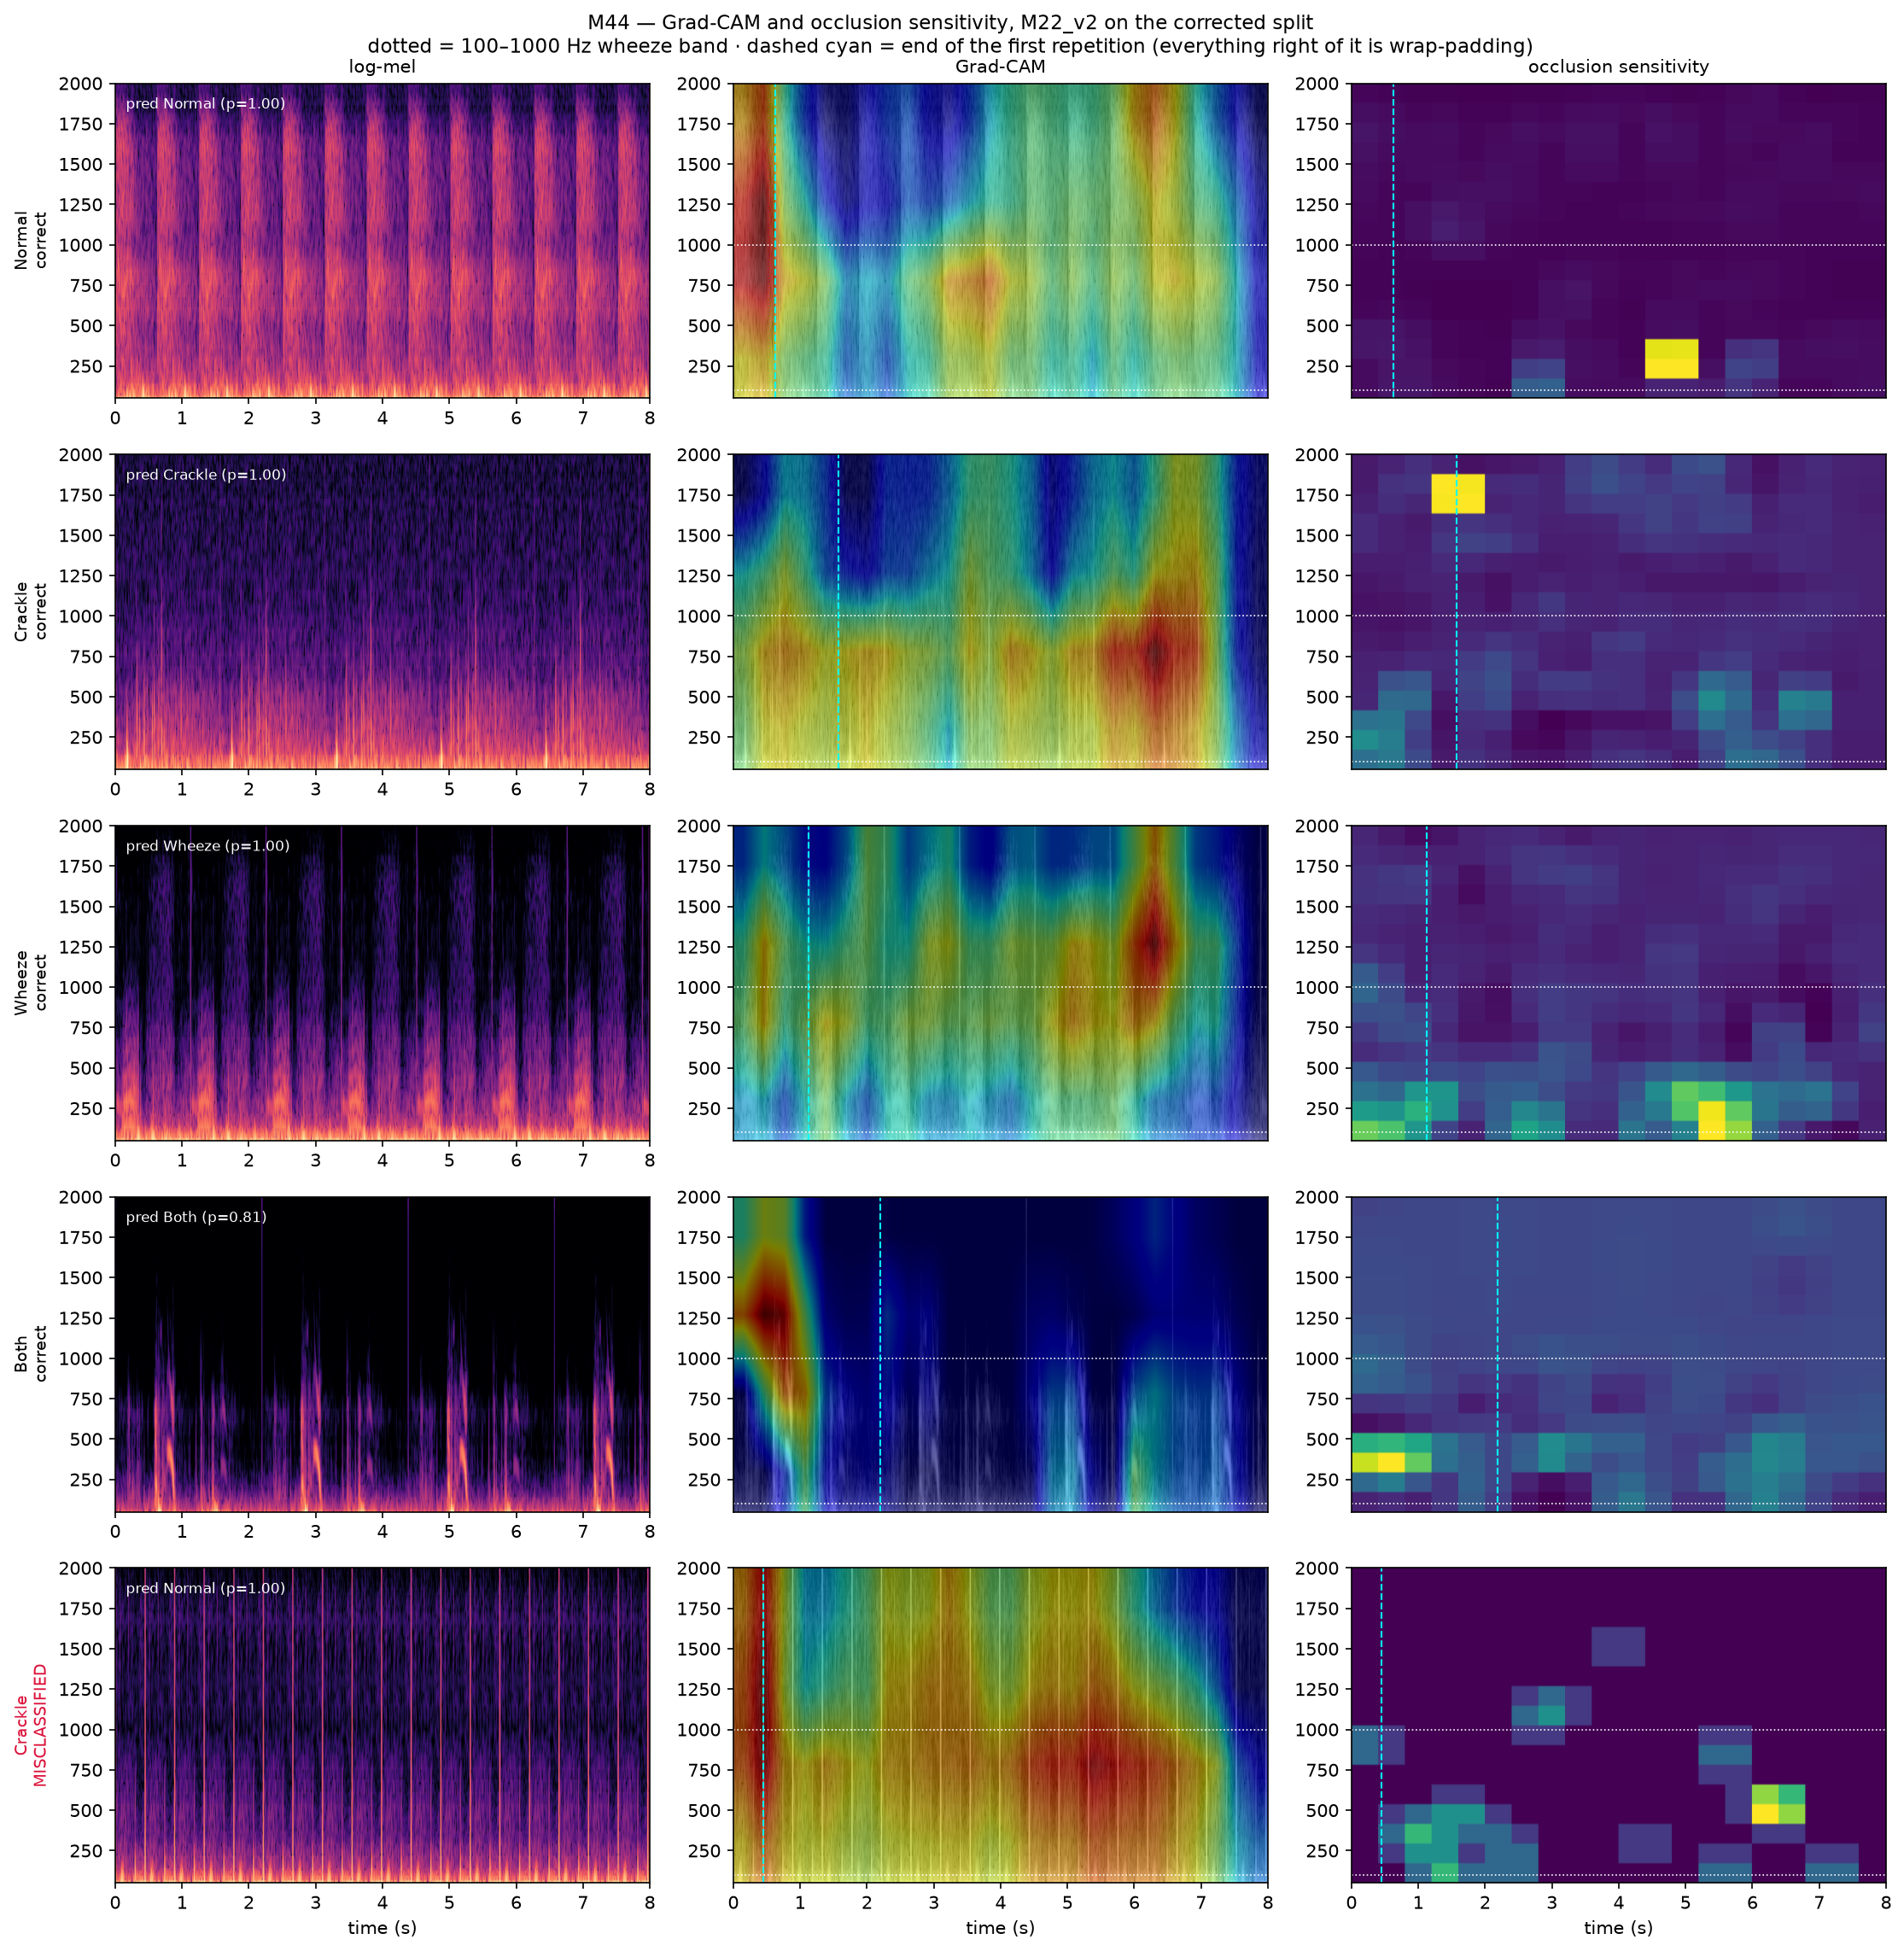
\includegraphics[width=0.95\linewidth]{figures/fig_xai_panels.png}
\caption{Attribution for the best model on the corrected partition. Each row shows
the log-mel input, the gradient-based class-activation overlay, the
occlusion-sensitivity map and the predicted versus true label. The bottom row is a
misclassification. Note the resolution caveat in Table~\ref{tab:xaiquant}: the
apparent fine structure in the activation maps is interpolation, not measurement.}
\label{fig:xai}
\end{figure}

\begin{table}[!t]
\centering
\caption{Quantitative interpretability measures on the best model, 400 test cycles
from the corrected partition. Both intervals exclude their null, so the
\emph{direction} of both results is trustworthy.}
\label{tab:xaiquant}
\small
\begin{tabular}{llrl}
\toprule
Measure & What it asks & Value & Reading \\
\midrule
Band pointing, wheeze present   & Share of attribution in 100--1000~Hz & 0.7140 & $n = 75$ \\
Band pointing, wheeze absent    & Same & 0.7674 & $n = 325$ \\
\best{Difference}               & Does a wheeze pull attention into the wheeze band? & \best{$-0.0534$} & [$-0.079$, $-0.026$], $p = 0.001$ \\
\quad uniform baseline          & & 0.5547 & \\
\midrule
Tiling consistency (mean $r$)   & Is attribution alike across identical repeated audio? & 0.098 & $n = 361$ \\
\quad fraction with $r > 0.5$   & & 0.3213 & \\
\midrule
Attribution on padded material  & Baseline model, cyclic tiling & \best{0.5938} & uniform share 0.6792 \\
\quad same, zero-padded model   & & 0.1013 & correctly ignores silence \\
\bottomrule
\end{tabular}

\vspace{2pt}
\footnotesize \textbf{Resolution caveat.} MobileNetV2 downsamples $32\times$, so the
final convolutional block is $4\times26$ cells---roughly 500~Hz and 0.31~s each.
Every activation map in Fig.~\ref{fig:xai} is that grid bilinearly upsampled. The
100--1000~Hz band spans about 1.8 of the 4 frequency cells, so band pointing is a
coarse contrast and not a localisation, and the maps must not be described as
showing the model ``focusing on'' fine structure. The occlusion maps use a
$16\times80$ patch at stride $8\times40$ and are better resolved; where the two
disagree, prefer occlusion.
\end{table}

Neither measure supports the reading that this model localises adventitious
sounds, and both are more informative for it.

\emph{The wheeze-band contrast runs backwards.} Both groups attend to the
physiological band above the uniform baseline, so the model does concentrate there
in general---but it attends \emph{less} to that band when a wheeze is actually
present. A wheeze detector should show the opposite sign.

\emph{The attribution is partly keyed to position rather than to sound.} The 8~s
input contains the same cycle tiled roughly three times, so a model reading
acoustics should attribute alike to each copy. It does not: mean correlation across
copies is 0.098, and only 32\% of cycles exceed 0.5. The padding experiment
sharpens this into the most uncomfortable number in the paper: the baseline model
places 59.4\% of its attribution on \emph{manufactured} audio---material created
by the tiling---while a zero-padded model correctly places 10.1\% of its
attribution on its padding. Cyclic tiling buys $+0.0311$ of official score
(Table~\ref{tab:ablation}, row \texttt{P4}) and costs attribution quality. We keep
it, because it is field-standard on this corpus and it wins on the reportable
metric, but the paper states that part of the gain is attributable to padding
structure rather than to respiratory acoustics.

We deliberately do \textbf{not} claim clinical interpretability from these maps. A
requested pointing-game analysis against annotated event windows is not
implementable on this corpus: ICBHI annotates one row per respiratory cycle and
marks whether the cycle contains an adventitious sound, not where inside it, and
our pipeline crops to exactly that window---so the annotated window \emph{is} the
model input and the hit rate is 100\% by construction. Reporting that number would
be reporting an artefact of the crop. Given that our own measurements put
clinician-versus-ICBHI agreement at $\kappa = 0.035$ on crackles, attributions
aligned to labels of that reliability cannot certify clinical reasoning. What
Table~\ref{tab:xaiquant} supports is a statement about where the model looks, and
that statement is negative.

\subsection{Error and Failure Analysis}
\label{subsec:errors}

\textbf{Research question: how does the system fail, and are the failures the same
kind?} Table~\ref{tab:errors} decomposes the best model's errors, and
Table~\ref{tab:failures} catalogues the project's outright run failures, because
both carry information a headline score does not.

\begin{table}[!t]
\centering
\caption{Error decomposition for the best model, from its raw confusion matrix.
Rows are true classes and the percentages are of that class's test cycles.}
\label{tab:errors}
\small
\begin{tabular}{lrrrrl}
\toprule
True class & Correct & $\rightarrow$ Normal & $\rightarrow$ Crackle & $\rightarrow$ other abnormal & Dominant error \\
\midrule
Normal  & 71.2\% & --- & 21.4\% & \phantom{0}7.5\% & Over-calls Crackle \\
Crackle & 51.9\% & 43.6\% & --- & \phantom{0}4.5\% & \best{Misses as Normal} \\
Wheeze  & 29.5\% & 47.7\% & 10.5\% & 12.3\% & \best{Misses as Normal} \\
Both    & 11.6\% & 37.2\% & 22.1\% & 29.1\% & \best{Misses as Normal} \\
\bottomrule
\end{tabular}

\vspace{2pt}
\footnotesize The single dominant failure mode is abnormal-to-Normal: 43.6\% of
Crackle, 47.7\% of Wheeze and 37.2\% of Both cycles are called Normal. This is the
same asymmetry the human studies report---seven senior physicians miss 77\% of
abnormal cycles~\cite{tzeng2025jmir}---and it is why a screening application must
be evaluated on $Se$ rather than on accuracy. Conversely, of the model's errors on
Normal cycles, 21.4\% are Crackle false alarms, which is the price the
class-weighted loss pays for the sensitivity it buys.
\end{table}

\begin{table}[!t]
\centering
\caption{Catalogue of run-level failures across the project, with the diagnostic
that caught each. Every one is reported rather than dropped; four are excluded
from all results tables and the reason is given.}
\label{tab:failures}
\small
\begin{tabular}{llll}
\toprule
Run & Failure mode & Diagnostic that caught it & Disposition \\
\midrule
M40 & Majority-class collapse & $Se = 0.0000$ under (\ref{eq:official}) & \best{Reported} as the small-data ViT finding \\
M33 & Normal-class collapse & $Sp = 0.0000$; macro metric hid it & Reported in Table~\ref{tab:extensions} \\
M36 & Majority-class collapse & $Se = 0.0932$ & Reported in Table~\ref{tab:extensions} \\
M35-v2 & Trained worse from update 1 & Best epoch 1 of 30 & Reported beside M35 \\
M21 & Majority-class collapse & $Se = 0.0186$; earlier version scored 1.000 & \best{Excluded} --- no train/test separation \\
M16, M18, M20 & Fitted and scored on the same rows & Recording-level, no split & \best{Excluded} \\
M30 & Score with no confusion matrix & Unverifiable, 0.8213 claimed & \best{Withdrawn} \\
M15 & Score with no confusion matrix & Reports 0.0000 & \best{Excluded} \\
M6, M14, M19 & Detection at or below chance & AUROC 0.4516 / 0.4809 / 0.3287 & Reported as negative results \\
M4 & No committed result record & Numbers exist only as prose & \best{Dropped} from every table \\
M43 & Never completed & --- & \best{\notrun}; no number reported \\
\bottomrule
\end{tabular}
\end{table}

Table~\ref{tab:failures} is unusual in a course report and we include it
deliberately. Nine of these twelve failures were caught by an automated check over
committed result records rather than by inspection, and three of the checks---
majority-class collapse, unverifiable score, and best-epoch-is-first---exist
because the corresponding failure actually occurred here. A pipeline that cannot
detect its own collapsed runs will report them as mediocre results, which is
exactly what the macro metric of (\ref{eq:macro}) was doing.

\subsection{Statistical Analysis}
\label{subsec:stats}

\textbf{Research question: which of the differences reported in this paper are
real?} Two things have to be established: how large run-to-run noise is, and what
the effective sample size of the test set is. Tables~\ref{tab:seedband}
and~\ref{tab:unit} answer them, and their answers point in opposite directions,
which is why both are reported.

\begin{table}[!t]
\centering
\caption{Noise floor: three runs of one identical configuration differing only in
the random seed.}
\label{tab:seedband}
\small
\begin{tabular}{lrrrrrr}
\toprule
 & Seed 42 & Seed 1 & Seed 2 & Mean & s.d. & Range \\
\midrule
ICBHI & 0.5540 & 0.5681 & 0.5657 & 0.5626 & \best{0.0075} & \best{0.0141} \\
\bottomrule
\end{tabular}

\vspace{2pt}
\footnotesize The published best model's 0.5602 sits inside this band, which is
also a reproducibility check: two independently written implementations of the
same recipe agree to within run-to-run noise. Reading
Table~\ref{tab:ablation}'s eleven deltas against the range, three do not clear it
(\texttt{A3}, \texttt{P1}, \texttt{P5}) and two clear it by less than $1.25\times$
(\texttt{A5}, \texttt{P3}); the remaining six clear it by $2.2\times$ or more.
\end{table}

\begin{table}[!t]
\centering
\caption{Unit of analysis. The same ten ablation rows tested twice against the
same baseline: exact McNemar over 2{,}636 paired cycle predictions, and a paired
bootstrap over the 47 test patients.}
\label{tab:unit}
\small
\begin{tabular}{lrrl}
\toprule
Row & Cycle-level $p$ (McNemar) & Patient-level 95\% CI & Verdict at patient level \\
\midrule
\texttt{A2} & $<10^{-15}$ & [$-0.130$, $+0.003$] & not shown to differ \\
\texttt{A3} & 0.150 & [$-0.049$, $+0.023$] & not shown to differ \\
\best{\texttt{A4}} & $<10^{-15}$ & \best{[$-0.154$, $-0.052$]} & \best{differs} \\
\texttt{A5} & 0.026 & [$-0.061$, $+0.020$] & not shown to differ \\
\texttt{A6} & $<10^{-15}$ & [$-0.092$, $+0.009$] & not shown to differ \\
\texttt{P1} & 0.128 & [$-0.059$, $+0.034$] & not shown to differ \\
\texttt{P2} & $7\times10^{-6}$ & [$-0.089$, $+0.011$] & not shown to differ \\
\texttt{P3} & 0.040 & [$-0.017$, $+0.046$] & not shown to differ \\
\texttt{P4} & $2.7\times10^{-5}$ & [$-0.068$, $+0.006$] & not shown to differ \\
\texttt{P5} & 0.428 & [$-0.041$, $+0.027$] & not shown to differ \\
\midrule
\multicolumn{2}{l}{\best{7 of 10 significant}} & \multicolumn{2}{l}{\best{1 of 10 significant --- 6 rows flip}} \\
\bottomrule
\end{tabular}
\end{table}

The disagreement in Table~\ref{tab:unit} is a finding, not a nuisance. Cycles
within a patient are not independent, so a cycle-level test answers a question
about 2{,}636 correlated draws and reports the answer as if they were 2{,}636
independent ones. \emph{The effective sample size of this ablation is 47, not
2{,}636.} An ablation table reporting cycle-level significance would have licensed
six conclusions this data does not support---and it would have looked more
rigorous than the table that does not.

Tables~\ref{tab:seedband} and~\ref{tab:unit} together are worth more than either
alone, and they do not contradict each other. The paired test says the 47-patient
test set is too small to certify most of the deltas; the seed band says run-to-run
noise is too small to explain them. The joint reading is that most of the effects
are probably real and \emph{this test set cannot establish them}. We report both
rather than choosing the one that flatters the table.

\subsection{Ablation Study}
\label{subsec:ablation}

\textbf{Research question: what is each component of the best model worth?}
Table~\ref{tab:ablation} is the leave-one-out ablation: twelve completed
one-variable experiments on the corrected partition, each paired against the
reference by a patient-level bootstrap.

\begin{table}[!t]
\centering
\caption{Component-wise and preprocessing ablation on the best model. One variable
changed per row, all on the corrected partition, 2{,}636 test cycles from 47
patients.}
\label{tab:ablation}
\small
\begin{tabular}{llrrlrrr}
\toprule
Row & Change from the full model & ICBHI & $\Delta$ & 95\% CI & $Se$ & $Sp$ & F1$_{\text{macro}}$ \\
\midrule
\texttt{A0} & Full model (reference)          & 0.5602 & ---       & [0.508, 0.614] & 0.4089 & 0.7115 & 0.4141 \\
\texttt{A1} & $-$ SpecAugment                 & 0.5200 & $-0.0402$ & [0.463, 0.575] & 0.4266 & 0.6135 & 0.3985 \\
\texttt{A2} & $-$ ImageNet initialisation     & 0.4999 & $-0.0603$ & [0.438, 0.551] & 0.3736 & 0.6263 & 0.3784 \\
\texttt{A3} & $-$ class-weighted loss         & 0.5497 & $-0.0105$ & [0.502, 0.593] & 0.4275 & 0.6718 & 0.4294 \\
\best{\texttt{A4}} & Frozen backbone, head only & \best{0.4595} & \best{$-0.1007$} & [0.400, 0.521] & 0.4349 & 0.4840 & 0.3374 \\
\texttt{A5} & 64 mel bins instead of 128      & 0.5427 & $-0.0175$ & [0.492, 0.587] & 0.4238 & 0.6615 & 0.4043 \\
\texttt{A6} & 4~s cycles instead of 8~s       & 0.5224 & $-0.0378$ & [0.463, 0.574] & 0.4954 & 0.5494 & 0.4058 \\
\midrule
\texttt{P4} & Zero-padding instead of tiling  & 0.5291 & $-0.0311$ & [0.478, 0.581] & 0.4684 & 0.5897 & 0.3841 \\
\texttt{P5} & $-$ spectrogram standardisation & 0.5539 & $-0.0063$ & [0.501, 0.604] & 0.4136 & 0.6942 & 0.4128 \\
\midrule
\multicolumn{8}{l}{\emph{Added stages --- read the sign in the opposite direction (see Table~\ref{tab:preproc})}}\\
\texttt{P1} & $+$ band-pass filter, 50--2000~Hz & 0.5513 & $-0.0089$ & [0.492, 0.601] & 0.4442 & 0.6583 & 0.4077 \\
\texttt{P2} & $+$ spectral-gating denoising   & 0.5248 & $-0.0354$ & [0.458, 0.588] & 0.4572 & 0.5923 & 0.3983 \\
\best{\texttt{P3}} & $+$ amplitude normalisation & \best{0.5764} & \best{$+0.0162$} & [0.514, 0.632] & 0.3996 & 0.7532 & 0.4217 \\
\bottomrule
\end{tabular}

\vspace{2pt}
\footnotesize Rows \texttt{A1}--\texttt{A6}, \texttt{P4} and \texttt{P5}
\emph{remove or replace} a stage the full model has; rows \texttt{P1}--\texttt{P3}
\emph{add} one it does not, so a positive delta there is a recommendation to adopt.
\textbf{Only row \texttt{A4} is shown to differ from the reference by the
patient-level paired test} (Table~\ref{tab:unit}). Rows \texttt{A0} and
\texttt{A1} are the two runs of Table~\ref{tab:augmentation}; the remaining ten
were run by a separate ablation harness whose reference configuration reproduces
\texttt{A0} to within the seed band of Table~\ref{tab:seedband}.
\end{table}

Table~\ref{tab:ablationreason} restates the same evidence in the form the
supervisor's reporting template asks for---one row per metric, two configurations,
the change, and the reason for it---using the largest and the most surprising
component as the two configurations.

\begin{table}[!t]
\centering
\caption{Ablation summary in per-metric form. Configuration A is the full model;
Configuration B freezes the backbone and trains the classifier only. The last
column is the part that carries the argument.}
\label{tab:ablationreason}
\small
\begin{tabular}{lrrrp{6.6cm}}
\toprule
Metric & Config.\ A & Config.\ B & Change & Possible reason \\
\midrule
ICBHI score & 0.5602 & 0.4595 & $-17.98\%$ & ImageNet features are not aligned with log-mel statistics; the transfer only pays once the backbone is allowed to move. \\
Sensitivity & 0.4089 & 0.4349 & $+6.36\%$ & The frozen model answers abnormal more often but with no discrimination, so the gain is a threshold shift, not detection. \\
Specificity & 0.7115 & 0.4840 & $-31.98\%$ & Almost the whole loss is here: without adaptation the model cannot represent what a normal cycle sounds like. \\
Accuracy & 0.5880 & 0.4640 & $-21.09\%$ & Tracks specificity, since Normal is 59\% of the test partition. \\
Precision (macro) & 0.4322 & 0.3391 & $-21.54\%$ & More abnormal answers spread over the same true positives. \\
F1 (macro) & 0.4141 & 0.3374 & $-18.52\%$ & Consistent with the precision loss; the minority classes degrade fastest. \\
Training time & 892~s & 451~s & $-49.44\%$ & Freezing halves the backward pass --- the only column where Configuration B wins. \\
\bottomrule
\end{tabular}
\end{table}

Three readings of the ablation are worth stating.

\emph{The single established component is fine-tuning.} Row \texttt{A4} is the only
row whose patient-level interval excludes zero, and
Table~\ref{tab:ablationreason} shows where its 0.10 goes: almost entirely into
specificity. A further row separates that effect from pretraining itself. Freezing
a \emph{randomly initialised} backbone scores 0.4979, statistically identical to
fine-tuning one (0.4999) since with no pretrained features there is nothing to
adapt---but frozen \emph{ImageNet} features score 0.4595, which is 0.038
\emph{below} frozen random features and $2.7\times$ the seed range.
\textbf{Frozen ImageNet representations are actively worse than random projections
on log-mel spectrograms.} That decomposes row \texttt{A4}'s $-0.1007$ into
``pretraining is worthless frozen'' plus ``adaptation is what the 0.10 buys'', and
neither ablation row alone could have produced it.

\emph{Of the three preprocessing stages our protocol specified and our pipeline
never implemented, only one helps.} Per-cycle amplitude normalisation gains
$+0.0162$; an explicit band-pass costs $-0.0089$, unsurprisingly, since the mel
filterbank's 50--2000~Hz limits already bound the band; and spectral-gating
denoising costs $-0.0354$. The denoising result is the caution worth reporting:
the stage a reviewer is most likely to ask for is the one that hurt most.

\emph{We decline to promote the highest row.} \texttt{P3}'s 0.5764 is the best
score in the table and our own pre-declared best-model rule nominally selects it.
Its patient-level interval spans zero, and its $+0.0162$ delta clears the seed band
of Table~\ref{tab:seedband} by less than $1.25\times$. A single unreplicated row
that is not shown to beat its own baseline is a lead, not a model. Amplitude
normalisation is worth adopting and re-running properly; it is not worth a
re-declaration on this evidence, and reporting the conflict rather than resolving
it silently is the point.

Table~\ref{tab:cumulative} answers a different question with the same runs. A
leave-one-out table asks what a component is worth \emph{given everything else}; a
cumulative ladder asks what it is worth \emph{given only what came before}. They
agree only when components do not interact, so both belong here.

\begin{table}[!t]
\centering
\caption{Cumulative ablation ladder: the baseline, then one component added per
rung. Both orderings are built from the same runs and differ only in which of two
components is added at rung 4, which makes the ordering effect measurable rather
than something to caveat.}
\label{tab:cumulative}
\small
\begin{tabular}{llccccrrr}
\toprule
Rung & Configuration & Pre-tr. & Fine-tune & Class wt. & SpecAug. & Amp.\ norm. & ICBHI & $\Delta$ \\
\midrule
\multicolumn{9}{l}{\emph{Order A --- SpecAugment added before class weighting}}\\
\texttt{S0} & Random init, frozen, plain CE & --- & --- & --- & --- & --- & \notrun & --- \\
\texttt{S1} & $+$ ImageNet pretraining & \checkmark & --- & --- & --- & --- & \notrun & --- \\
\texttt{S2} & $+$ full fine-tuning & \checkmark & \checkmark & --- & --- & --- & \notrun & --- \\
\texttt{S3} & $+$ SpecAugment & \checkmark & \checkmark & --- & \checkmark & --- & 0.5497 & --- \\
\texttt{S4} & $+$ class-weighted CE & \checkmark & \checkmark & \checkmark & \checkmark & --- & 0.5602 & $+0.0105$ \\
\texttt{S5} & $+$ amplitude normalisation & \checkmark & \checkmark & \checkmark & \checkmark & \checkmark & \best{0.5764} & $+0.0162$ \\
\midrule
\multicolumn{9}{l}{\emph{Order B --- class weighting added before SpecAugment}}\\
\texttt{S3} & $+$ class-weighted CE & \checkmark & \checkmark & \checkmark & --- & --- & 0.5200 & --- \\
\texttt{S4} & $+$ SpecAugment & \checkmark & \checkmark & \checkmark & \checkmark & --- & 0.5602 & $+0.0402$ \\
\texttt{S5} & $+$ amplitude normalisation & \checkmark & \checkmark & \checkmark & \checkmark & \checkmark & \best{0.5764} & $+0.0162$ \\
\bottomrule
\end{tabular}

\vspace{2pt}
\footnotesize \textbf{Rows \texttt{S0}--\texttt{S2} had not completed at
submission and are written \notrun\ rather than filled with a plausible value};
filling them would be exactly the fault this paper is about, committed knowingly.
\textbf{The ordering effect is the point of showing both halves.} SpecAugment is
credited with $+0.0402$ when it is added after class weighting and class weighting
with $+0.0105$ when it is added after SpecAugment---so the two interact, and a
single cumulative table would have silently claimed its own ordering was the
natural one. Compare with Table~\ref{tab:ablation}, where the leave-one-out deltas
for the same two components are $-0.0402$ and $-0.0105$.
\end{table}

\subsection{Why the Gap Is Where It Is}
\label{subsec:pretraining}

Before comparing against published work, it is worth naming what the comparison
will show and why, because the five measurements collected in
Table~\ref{tab:gapevidence} converge on one answer and it is not architecture.

\begin{table}[!t]
\centering
\caption{Five convergent measurements on the source of the performance gap. Four
are from this work.}
\label{tab:gapevidence}
\small
\begin{tabular}{llp{8.2cm}}
\toprule
\# & Source & Evidence \\
\midrule
1 & Literature (Table~\ref{tab:comparison}) & Every published method above 0.57 uses an audio-domain-pretrained backbone; every method below uses hand-crafted features or an ImageNet vision network. \\
2 & Literature~\cite{frozenfm2025} & A \emph{frozen} AudioSet encoder with a linear head scores 0.5938 --- above every model we fully fine-tuned. \\
3 & \best{This work}, Table~\ref{tab:main} & Our ImageNet ViT-B/16 (86~M), Swin-T (27.5~M) and DeiT-S (21.7~M) all lose to our ImageNet MobileNetV2 (2.2~M). Twelve to thirty-eight times the parameters, a worse score. \\
4 & \best{This work}, Table~\ref{tab:ablation} & Removing ImageNet initialisation costs $-0.0603$, and frozen ImageNet features score \emph{below} frozen random ones. \\
5 & \best{This work}, Table~\ref{tab:ceiling} & A frozen AudioSet network that never heard a stethoscope reaches 0.7115 / 0.7621 on the same cycles our detectors failed on at 0.5580 / 0.5729. \\
\bottomrule
\end{tabular}
\end{table}

Rows 3 and 4 are a clean, ImageNet-controlled architecture sweep---one
convolutional network against three vision transformers, one variable---and the
ICBHI literature does not contain it, because nobody publishes ImageNet-only
transformers on this corpus any more. \emph{The transformer era on this benchmark
is an audio-pretraining era wearing a transformer label}, and our M40--M42 runs are
the ablation that separates the two. The ViT collapse belongs to this story rather
than being an embarrassment: 86~M parameters, 4{,}251 training cycles, no in-domain
prior. It is also the strongest argument for completing the AST run of
Table~\ref{tab:models}, which is the one experiment that would test the hypothesis
directly, and its absence is stated as a limitation rather than papered over.

\subsection{Comparison with Existing Works}
\label{subsec:comparison}

Table~\ref{tab:comparison} places this work against the literature. We report the
official metric only, and we report the partition for every row, because the
argument of this paper is that a comparison without those two columns is not a
comparison.

\begin{table}[!t]
\centering
\caption{Comparison of the proposed system with existing work on ICBHI 2017. All
scores are the official challenge metric of (\ref{eq:official}). Rows are grouped
by partition, and rows from different groups are not rankable against one another.}
\label{tab:comparison}
\small
\begin{tabular}{lllrrr}
\toprule
Author & Dataset & Network & $Se$ & $Sp$ & \best{ICBHI} \\
\midrule
\multicolumn{6}{l}{\emph{Published 60/40 partition, official metric --- directly comparable}}\\
Gairola \emph{et al.}~\cite{respirenet2021} & ICBHI 2017 & ResNet34, ImageNet & 0.401 & 0.723 & 0.5620 \\
Moummad and Farrugia~\cite{scl2023} & ICBHI 2017 & CNN6, supervised contrastive & 0.392 & 0.760 & 0.5755 \\
Niizumi \emph{et al.}~\cite{frozenfm2025} & ICBHI 2017 & M2D, \emph{frozen} linear probe & 0.466 & 0.722 & 0.5938 \\
Bae \emph{et al.}~\cite{bae2023patchmix} & ICBHI 2017 & AST, patch-mix contrastive & 0.431 & 0.817 & 0.6237 \\
Kim \emph{et al.}~\cite{bts2024} & ICBHI 2017 & CLAP, BTS & 0.457 & 0.814 & 0.6354 \\
Jeong \emph{et al.}~\cite{pafa2025} & ICBHI 2017 & BEATs, PAFA & 0.476 & 0.821 & \best{0.6484} \\
Tzeng \emph{et al.}~\cite{tzeng2025jmir} & ICBHI 2017 & 7 senior physicians & 0.232 & 0.723 & 0.4777 \\
\addlinespace
\best{This work} & ICBHI 2017 & MobileNetV2 + SpecAugment & 0.456 & 0.672 & \best{0.5641} \\
\best{This work} & ICBHI 2017 & MobileNetV3-Small & 0.198 & 0.828 & 0.5132 \\
\best{This work} & ICBHI 2017 & 2D-CNN, from scratch & 0.201 & 0.744 & 0.4720 \\
\midrule
\multicolumn{6}{l}{\emph{Corrected patient-independent partition --- not comparable to the block above}}\\
\best{This work} & ICBHI 2017 & MobileNetV2 + SpecAugment & 0.409 & 0.712 & \best{0.5602} \\
\best{This work} & ICBHI 2017 & Swin-T & 0.343 & 0.718 & 0.5304 \\
\best{This work} & ICBHI 2017 & MobileNetV2, no augmentation & 0.427 & 0.614 & 0.5200 \\
\best{This work} & ICBHI 2017 & ViT-B/16 (collapsed) & 0.000 & 0.999 & 0.4994 \\
\midrule
\multicolumn{6}{l}{\emph{Identifier-fallback partition --- reported only to price the fault}}\\
This work & ICBHI 2017 & MobileNetV2 + SpecAugment & 0.570 & 0.729 & 0.6495 \\
This work & ICBHI 2017 & \emph{the same run, macro metric} & 0.570 & 0.729 & 0.7077 \\
\bottomrule
\end{tabular}

\vspace{2pt}
\footnotesize Published rows are the official partition, 2{,}756 test cycles from
49 patients; our first block is the identical partition and metric, which is why it
is the only block of ours that may be read against them. Two works cited elsewhere
in this paper are deliberately absent because they do not report a number this
table can hold: Suma \emph{et al.}~\cite{suma2025mtl} report accuracy on an
unstated partition, and Cho and Lee~\cite{cho2025openset} report an improvement
over a semi-supervised baseline rather than an absolute score. Excluding them is
this paper's own argument applied to its own table.
\end{table}

Read on the partition the literature actually uses, our best model reaches 0.5641.
That places it above RespireNet, the strongest ImageNet-pretrained convolutional
system in the table, and below every audio-pretrained one, 8.4 points short of the
strongest system shown.

The composite score, however, conceals the more informative comparison, and this
is the concrete payoff of the reporting discipline of
Section~\ref{subsec:protocol}. \emph{Our sensitivity is not behind the field at
all.} At 0.456 it exceeds RespireNet (0.401), supervised contrastive pretraining
(0.392) and patch-mix contrastive learning (0.431), and is level with BTS (0.457),
trailing only the frozen probe (0.466) and PAFA (0.476). The entire deficit is
specificity: 0.672 against a field spanning 0.722 to 0.821. We are not uniformly
weaker; we occupy a different operating point, detecting abnormal cycles at the
field's rate while over-calling them on normal ones---the direction a
class-weighted loss and SpecAugment push a model by design, and arguably the
direction a screening application should prefer, though the challenge metric does
not reward it. Under the composite alone the distinction disappears entirely.

The last two rows of Table~\ref{tab:comparison} are the ones the paper exists for.
Our unaudited pipeline reported 0.7077. That number would have placed \emph{first}
in this table, ahead of every published system in it, on a partition covering 7.1\%
of the corpus under a metric we had defined ourselves. It is not state of the art;
it is an unaudited measurement. A 2.23~M-parameter MobileNetV2 matching a 2021
EMBC ResNet34 is an honest outcome for a course project, and the contribution was
never the number.

\subsection{Limitations}
\label{subsec:limitations}

Eight limitations bound the claims above, and the first is the most serious.

\emph{Checkpoint selection reads the test partition.} The corrected-partition runs
of Table~\ref{tab:main} and every ablation row select the saved epoch on the test
score, because no separate validation split was carved out of the 79 training
patients. This is optimistic, and it is equally optimistic for every row, so the
within-table comparisons, the seed band and the ablation deltas are unaffected---but
the absolute numbers are not clean held-out estimates and must not be read as
such. The two backbones that \emph{did} carve out a validation split (M2 and M3 in
the second block of Table~\ref{tab:efficiency}, 12 held-out patients, test read
once) score 0.4720 and 0.5132, which is the right order of magnitude but not a
controlled comparison. Repairing this for the whole suite is the single highest-value
remaining run.

\emph{The split effect is measured for one model, not for the suite.} Only the best
model was run on all three treatments of the partition. The two other backbones
that appear on both the fallback and the corrected partition changed architecture
between runs---a five-block scratch network became a four-block one, and a
MobileNetV2 became a MobileNetV3-Small---so their apparent split effects of
$-0.1418$ and $-0.0763$ are confounded with architecture and are \emph{not} quoted
as split measurements anywhere in this paper. Only the $-0.0854$ and $-0.0039$
figures of Table~\ref{tab:protocol} are one-variable measurements.

\emph{The fourth transformer is missing.} The plan called for four transformer
backbones, one per member, and the fourth---the only audio-domain-pretrained
one---did not complete. Its absence is precisely where the argument of
Section~\ref{subsec:pretraining} would have been tested rather than inferred.

\emph{The ablation reference is not byte-identical to the best model.} Two of the
twelve ablation rows come from the best model's own notebook and ten from a
separate harness whose reference configuration reproduces the best model to within
the seed band of Table~\ref{tab:seedband}, but not exactly; the harness also
reports a slightly different parameter count. The seed band is what licenses
treating them as one table, and we state the wrinkle rather than hide it.

\emph{Three rungs of the cumulative ladder are missing}, so Table~\ref{tab:cumulative}
cannot yet price pretraining and fine-tuning in cumulative form.

\emph{The human side rests on one rater.} Our clinician study has $n=1$ against the
$n=7$ and $n=12$ of the cited literature, so no inter-rater agreement is computable
from it. Its intra-rater reliability is measured and substantial, and its
sensitivity replicates the published seven-physician figure to within a tenth of a
point, but a single rater is a single rater. The listening pack is also not a
random sample---cycles under 0.9~s were excluded and each stratum sorted
longest-first---so the absolute levels in Table~\ref{tab:sameclips} are not
comparable to corpus-wide numbers, and only the paired contrast is.

\emph{The probe result bounds a learned detector, not a hand-built one.}
Table~\ref{tab:ceiling} shows these labels are learnable at 0.71--0.87. It does not
show that an \emph{interpretable, non-learned} concept detector can reach 0.65 on
them, and the probe itself is linear and single-recipe. The practical ceiling for
physics-derived concept detection on this corpus remains open.

\emph{One corpus.} The faults described here are ICBHI-specific and the scope of the
claim is that benchmark and no further. Extending the audit to other corpora is the
obvious next step and is not attempted here.

%=======================================================================
\section{Conclusions}
\label{sec:conclusion}

We audited our own respiratory sound pipeline on the ICBHI 2017 database and found
five measurement faults, then priced each rather than assuming they mattered
equally. A macro-averaged variant of the challenge score inflated twenty committed
runs by 0.0948 on average and 0.2176 at worst, and masked two outright model
collapses that the official metric exposes immediately. A silent partition fallback
substituted an eleven-patient, 7.1\% test set for the official 40\% one, worth
0.0854 on the best model. The published official partition assigns recordings
rather than patients and is not patient-independent, placing 4.4\% of its test
cycles---and 40\% of its rarest class---in patients the model may have trained on;
repairing that leak moved the score by only 0.0039, so we report it as a validity
fault and explicitly not as a source of inflation. The same partition file names a
recording whose device suffix does not match the released audio, so a naive join
discards it in silence. And selecting the saved checkpoint on the loss rather than
on the challenge score costs 0.075 to 0.102 across three seeds, more than any
architectural component in the paper. Ranking the faults honestly is part of the
contribution: two change the number materially, one is worth nothing, one destroys
data quietly, and one is larger than the modelling choices it hides behind.

Under the corrected protocol we reported a full model suite with its complete
metric, size and timing record; a paired augmentation study showing that
SpecAugment is worth $+0.0402$ on a convolutional backbone and nothing on three
transformers; a twelve-row ablation in which only one component---fine-tuning the
backbone---is established by a patient-level paired test; a cumulative ladder that
measures its own ordering effect; a three-seed noise floor; and attribution
analysis showing that the best model attends \emph{less} to the wheeze band when a
wheeze is present and places 59\% of its evidence on audio the padding scheme
manufactured. We also reported a pre-registered concept-validity gate, run twice
and failed twice under a threshold chosen so that it \emph{could} fail, and then
retracted our own reading of that failure: a probe on a frozen general-audio
representation that has never heard a stethoscope reaches 0.71 and 0.76 on the same
cycles, so the labels are learnable and our detectors were weak. What replaces the
retracted claim is sharper---a self-consistent physician agrees with these same
cycle labels at $\kappa = 0.035$ on crackles, and on matched clips the machine
reproduces the reference standard significantly better than the physician does for
wheeze. We withdrew two further results of our own: an interpretability cost
recorded from a single random initialisation that reverses sign across five, and a
mechanism verdict produced by a sign test whose design floor made it incapable of
ever supporting the hypothesis. The contribution is a measurement rather than a
mechanism, and we release the corrected split loader, the canonical score format
with paired significance tests, and the audit tool that detects every fault
described here.

Three directions follow. \emph{First}, carve a validation split out of the training
patients and re-run the suite, so that the absolute numbers become clean held-out
estimates and the checkpoint-selection fault is closed rather than merely priced;
the same exercise would complete the three missing rungs of the cumulative ladder
and settle whether the operating-point difference we report against the literature
is a property of this backbone and loss or of the corrected partition itself.
\emph{Second}, run the audio-domain-pretrained transformer the plan called for and
never completed, which is the one experiment that would test the pretraining
hypothesis of Section~\ref{subsec:pretraining} directly rather than by convergent
inference from five indirect measurements. \emph{Third}, apply the audit outward: the
five fault classes described here are each detectable from a committed confusion
matrix and a stated partition, and a survey of how many published ICBHI systems
supply either would establish whether these are our errors or the field's.

%=======================================================================
\bibliographystyle{IEEEtran}
\bibliography{references}

\end{document}
